%%%%%%%%%%%%%%%%%%%%%%%%%%%%%%%%%%%%%%%%%%%%%%%%%%%%%%%%%%%%%%%%%%%%%%%%%%%%%%%%
% event_selection.tex: 
%%%%%%%%%%%%%%%%%%%%%%%%%%%%%%%%%%%%%%%%%%%%%%%%%%%%%%%%%%%%%%%%%%%%%%%%%%%%%%%%
\chapter{Event Selection}
\label{sec:event_selection_chapter}
%%%%%%%%%%%%%%%%%%%%%%%%%%%%%%%%%%%%%%%%%%%%%%%%%%%%%%%%%%%%%%%%%%%%%%%%%%%%%%%%

The LRS model predicts the existence of a \WR and \nul that decay to two energetic charged leptons and two 
energetic jets.  Using the 2.6 fb$^{-1}$ \cite{lumi} of data recorded by CMS from September through November 
2015, evidence of a \WR and \nul was searched for in events with $eejj$ and $\mu\mu jj$ final states.  
Events were selected using requirements that were developed based on features of ST processes and \WR and \nul 
decays.


\section{Selections based on \WR signal and ST backgrounds}
\label{sec:signalAndBkgndFeatures}
The event selections were driven by model independent features of \WR and \nul decays and ST processes in the $\ell\ell jj$ 
final states.  The expected \WR mass (\mWR) was large, above 2 $\TeV$, relative to the 13 $\TeV$ collision energy, 
so \WR bosons were expected to have low net momentum.  Therefore, the charged lepton and jet decay 
products, on average, were distributed uniformly in $\phi$, and concentrated in the $|\eta| < 2.4$ 
region\footnote{The $|\eta| < 2.4$ region covers 94\% of the $0 \leq \theta < 180$ degree phase space, where 
$\theta = 0$ points along the beam axis.}, 
as shown in Figures \ref{fig:wrLeptonEtas} and \ref{fig:wrJetEtas}.  Furthermore, the large expected 
\mWR meant final state leptons and jets would have $\pt$ of several hundred $\GeV$ or more, as shown in 
Figures \ref{fig:wrLeptonPts} and \ref{fig:wrJetPts}.  In contrast, the ST backgrounds 
produced leptons and jets primarily with $\pt < 100$ $\GeV$, as shown in Figures \ref{fig:bkgLeptonPts} 
and \ref{fig:bkgJetPts}.  These kinematic features motivated the event selections:

\begin{itemize}
	\item Two leptons were reconstructed with $\pt > 53$ $\GeV$, and one had $\pt > 60$ $\GeV$.
	\item Two jets were reconstructed with $\pt > 40$ $\GeV$.
	\item Both leptons and jets were reconstructed with $|\eta| < 2.4$.
	\item The invariant mass $\Mlljj$ of the reconstructed leptons and jets exceeded $\Mlljj > 600$ $\GeV$.
\end{itemize}

The large expected mass difference between a charged lepton $\ell$ and a \nul motivated 
additional event selections.  In the $\WR \rightarrow \ell_{1} \nul$ decay, the $\ell_{1}$ recoiled against 
the heavier \nul to conserve momentum.  Then, the \nul decayed to 
a second lepton $\ell_{2}$ and two jets that recoiled against the $\ell_{1}$.  
Thus the lepton pair $\ell_{1}\ell_{2}$, on average, had a large dilepton mass ($\Mll$, Table \ref{tab:wrMll}), 
and the $\ell_{1}$ was well separated from the \nul decay products.  In constrast, \DY and diboson (WW, WZ, ZZ) 
events primarily had $\Mll < 180 \GeV$.  In $\WR \rightarrow \ell_{1} \nul$ decays, 
the neutrino masses $\mnul$ are expected to exceed the ST $Z$ boson mass in order to predict ST neutrino 
masses below 1 eV consistent with experimental evidence \cite{sumNuMassLimit}, and to suppress left-right 
mixing, which increases \nul production through $pp \rightarrow Z \rightarrow \nu\nu \rightarrow \nul\nu$.  
The high expected $\mnul$ resulted in large $\Delta R$ separations between \nul decay products.  However, 
in QCD and other multi-jet events with a reconstructed lepton, the lepton was often a byproduct of 
hadronization, and was reconstructed near a jet but not clustered into it.  The separation between leptons 
and jets, and the recoil of the $\ell_{2}$ against the $\ell_{1}$ motivated the additional event selections:

\begin{itemize}
	\item Each reconstructed lepton was separated from the other lepton and both jets by $\Delta R > 0.4$.
	\item The dilepton mass $\Mll$ of the two reconstructed leptons exceeded $\Mll > 200$ $\GeV$.
\end{itemize}


\begin{figure}[btp]
	\centering
	\subfigure{
		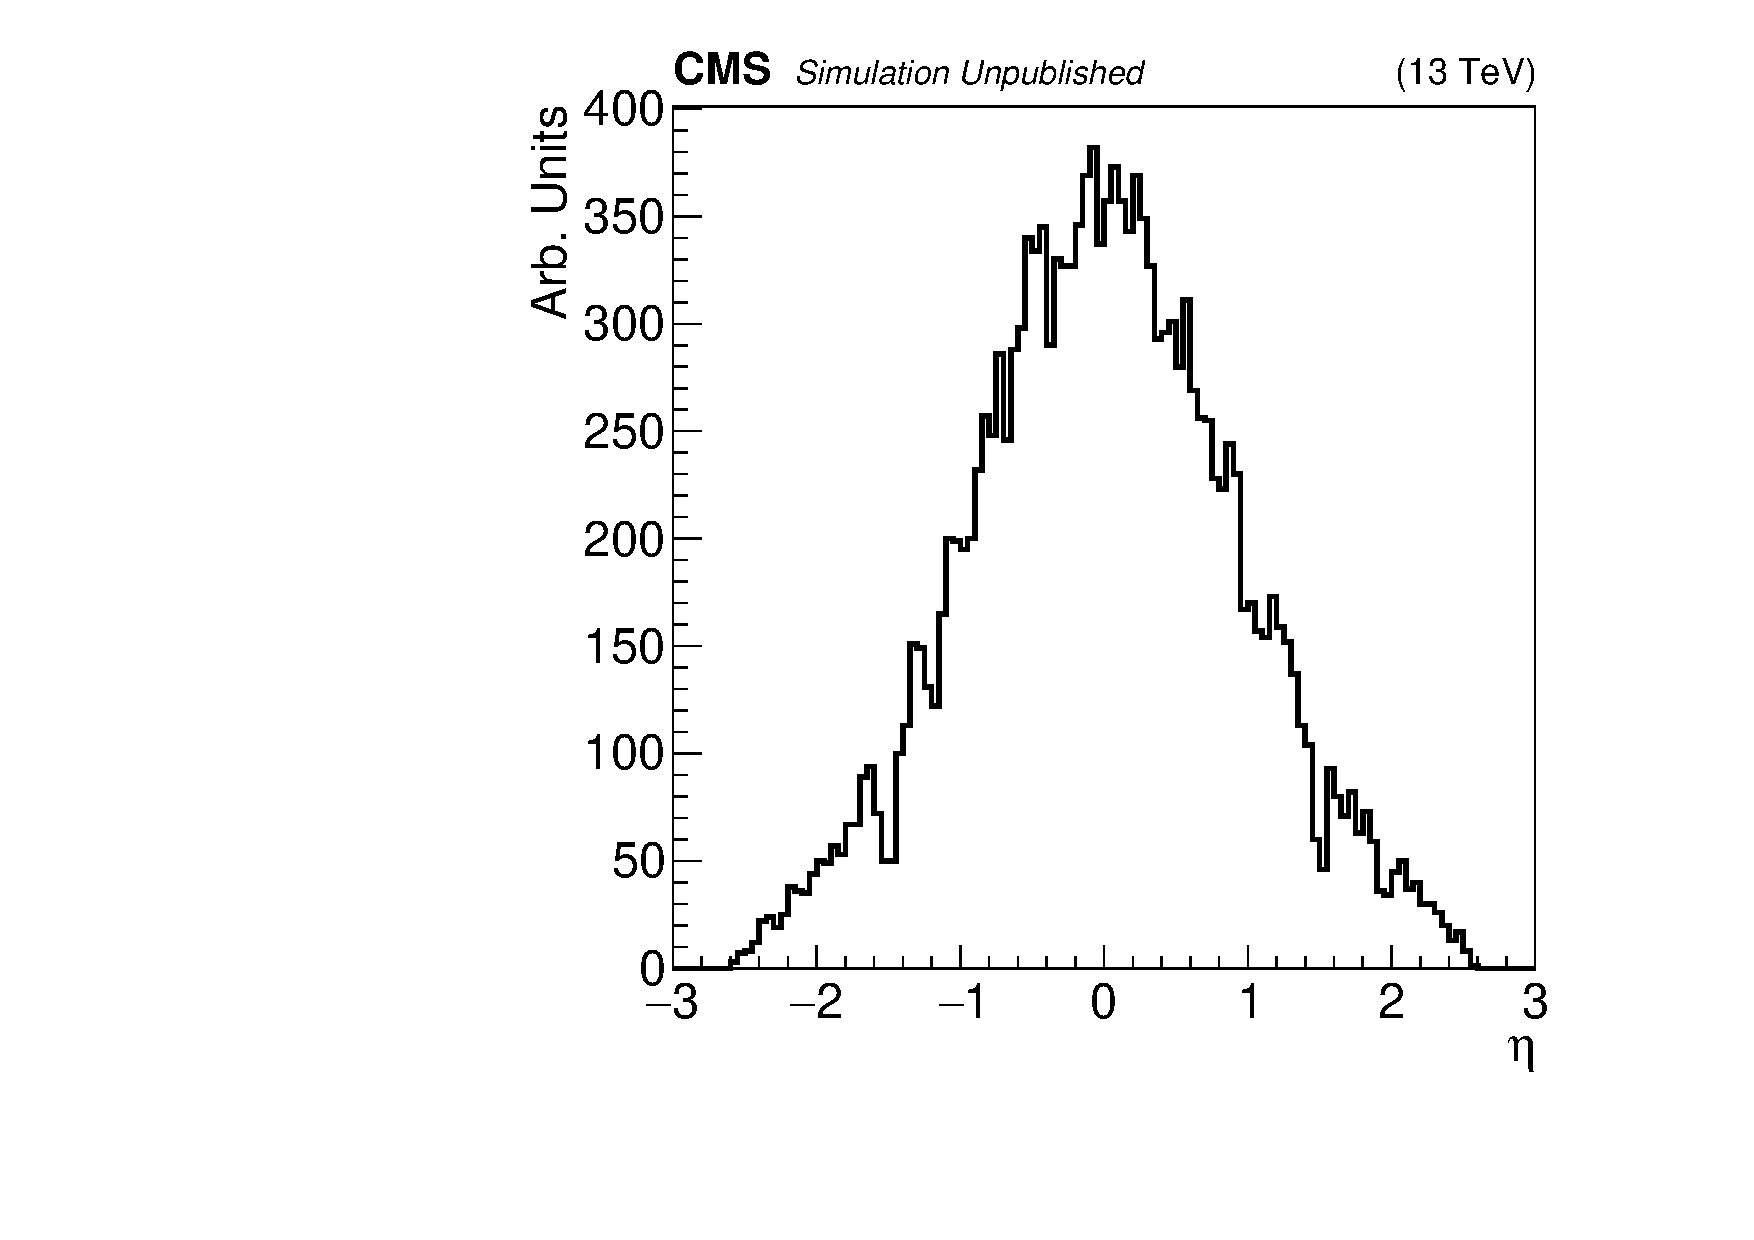
\includegraphics[width=0.65\textwidth]{figures/etaMatchedRecoEleFromWr_mwr2200_mnu1100.pdf}
	}
	\subfigure{
		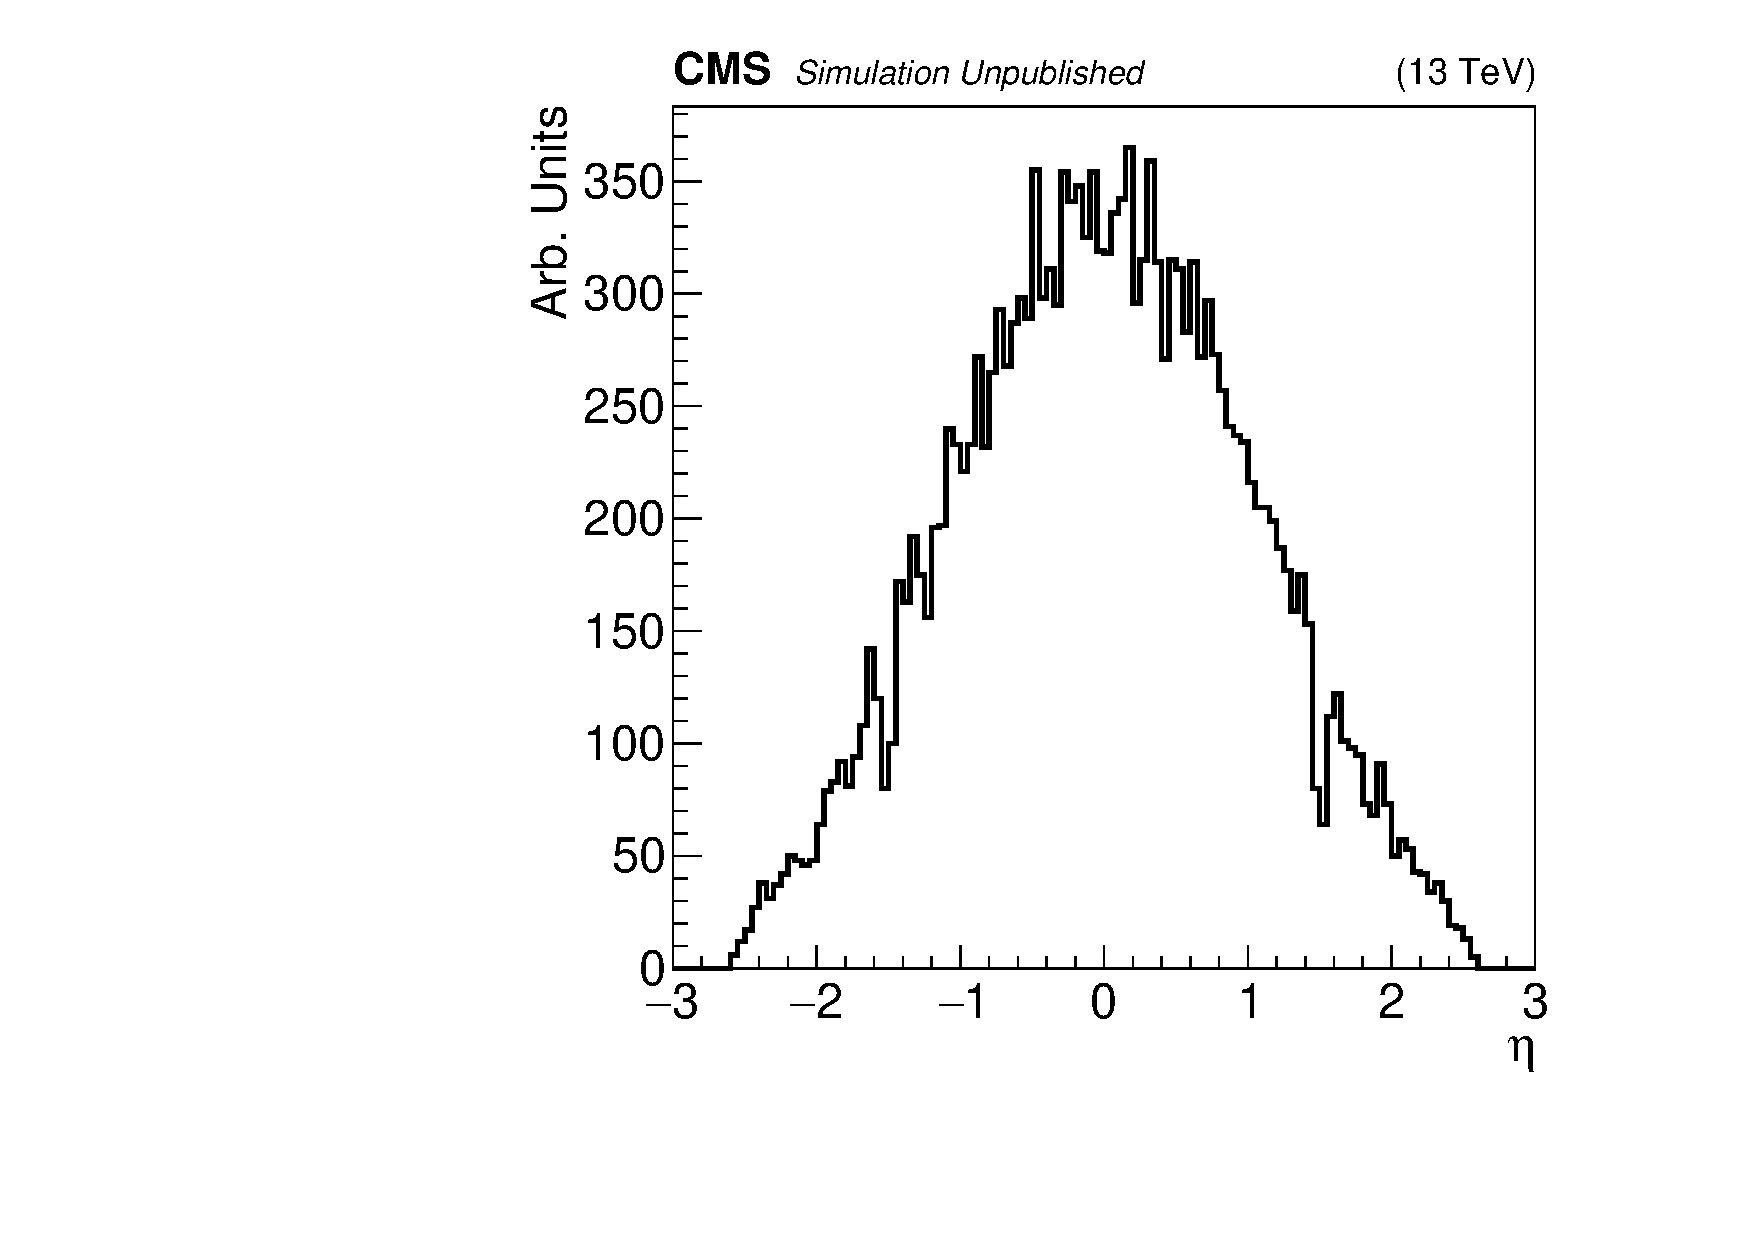
\includegraphics[width=0.65\textwidth]{figures/etaMatchedRecoEleFromNu_mwr2200_mnu1100.pdf}
	}
	\label{fig:wrLeptonEtas}
	\caption{The $\eta$ distribution of the reconstructed electron produced by the \WR (\nul) decay is shown on the top (bottom) for 
		simulated $\WR \rightarrow eejj$ events with $\mWR = 2.2 \TeV$ and $\mnul = 1.1 \TeV$.}
\end{figure}

\begin{figure}[btp]
	\centering
	\subfigure{
		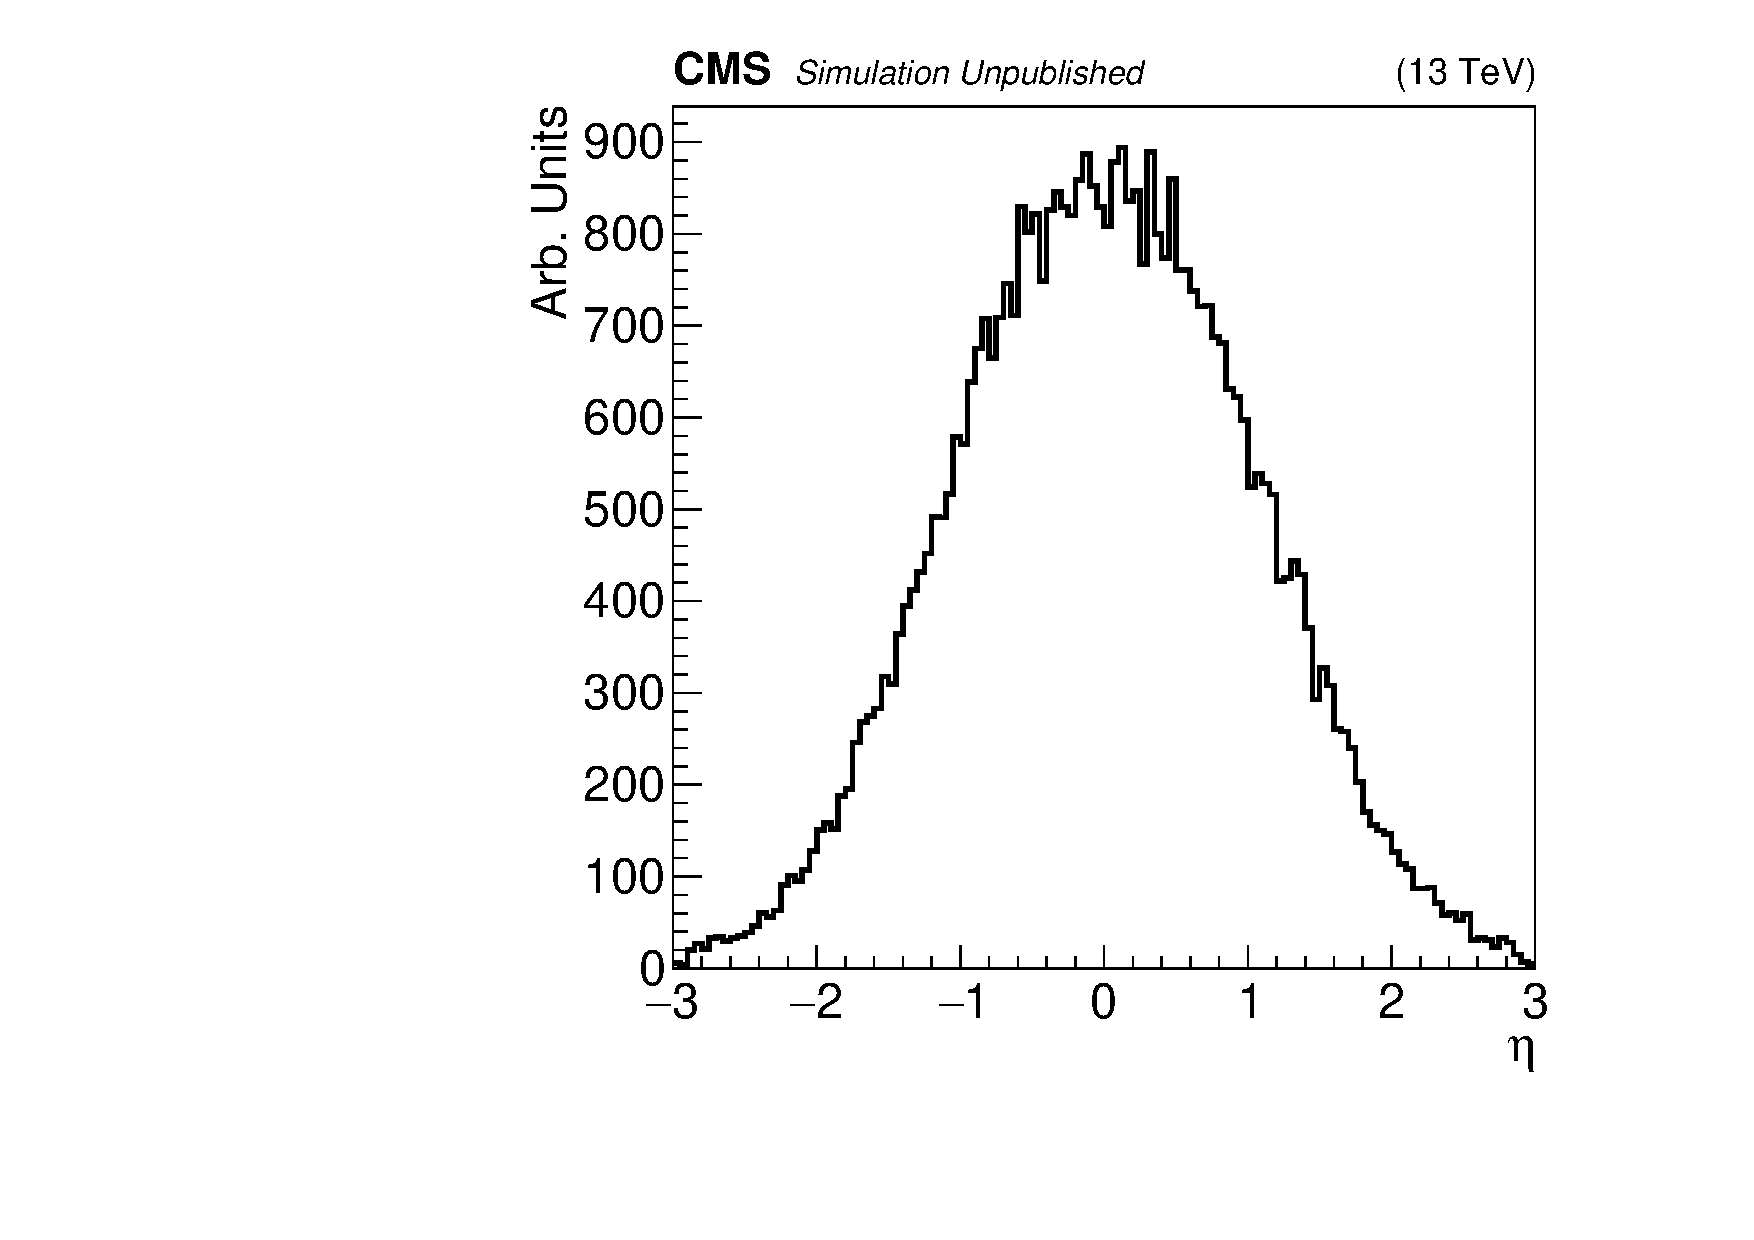
\includegraphics[width=0.65\textwidth]{figures/etaMatchedRecoJetOne_mwr2200_mnu1100.pdf}
	}
	\subfigure{
		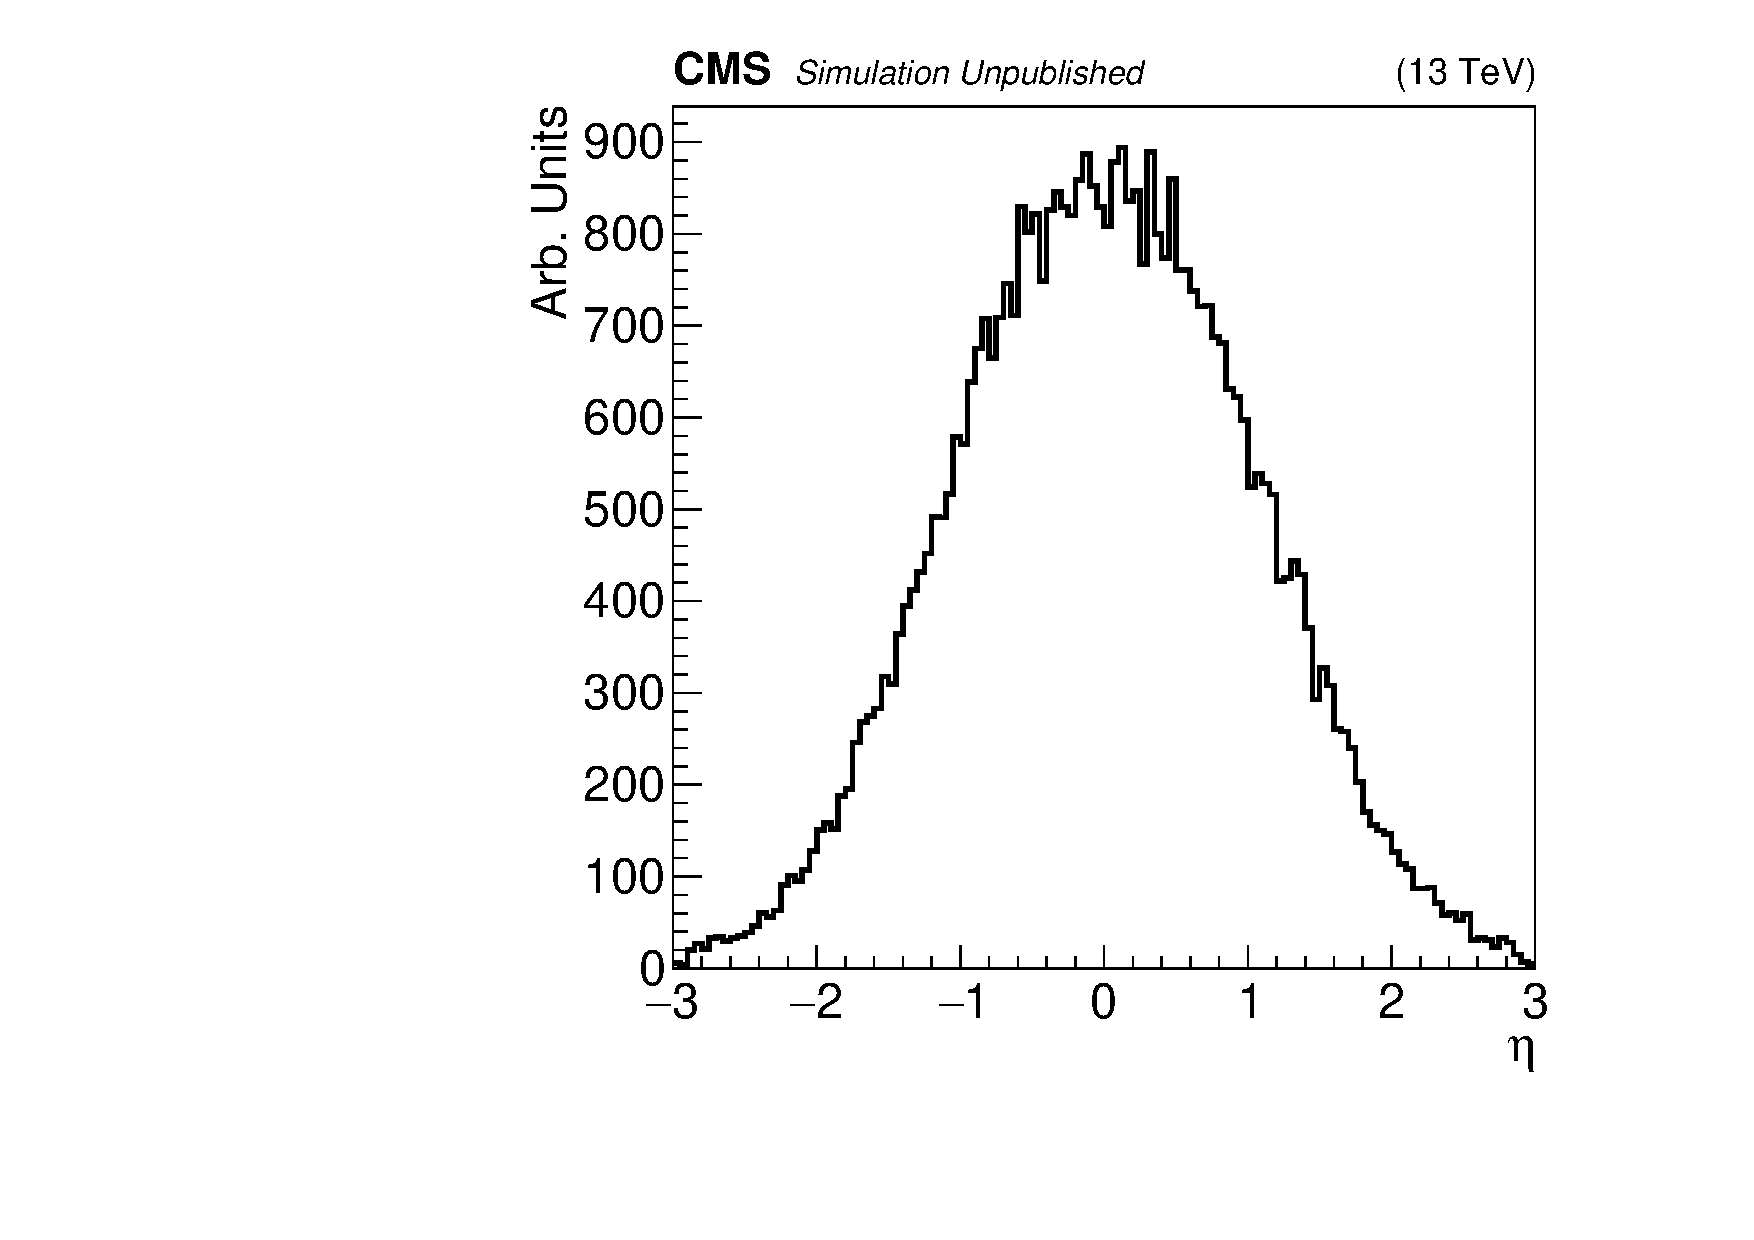
\includegraphics[width=0.65\textwidth]{figures/etaMatchedRecoJetOne_mwr2200_mnu1100.pdf}
	}
	\label{fig:wrJetEtas}
	\caption{The $\eta$ distributions of the reconstructed jets produced by the \nul decay are shown for 
		simulated $\WR \rightarrow eejj$ events with $\mWR = 2.2 \TeV$ and $\mnul = 1.1 \TeV$.}
\end{figure}

\begin{figure}[btp]
	\centering
	\subfigure{
		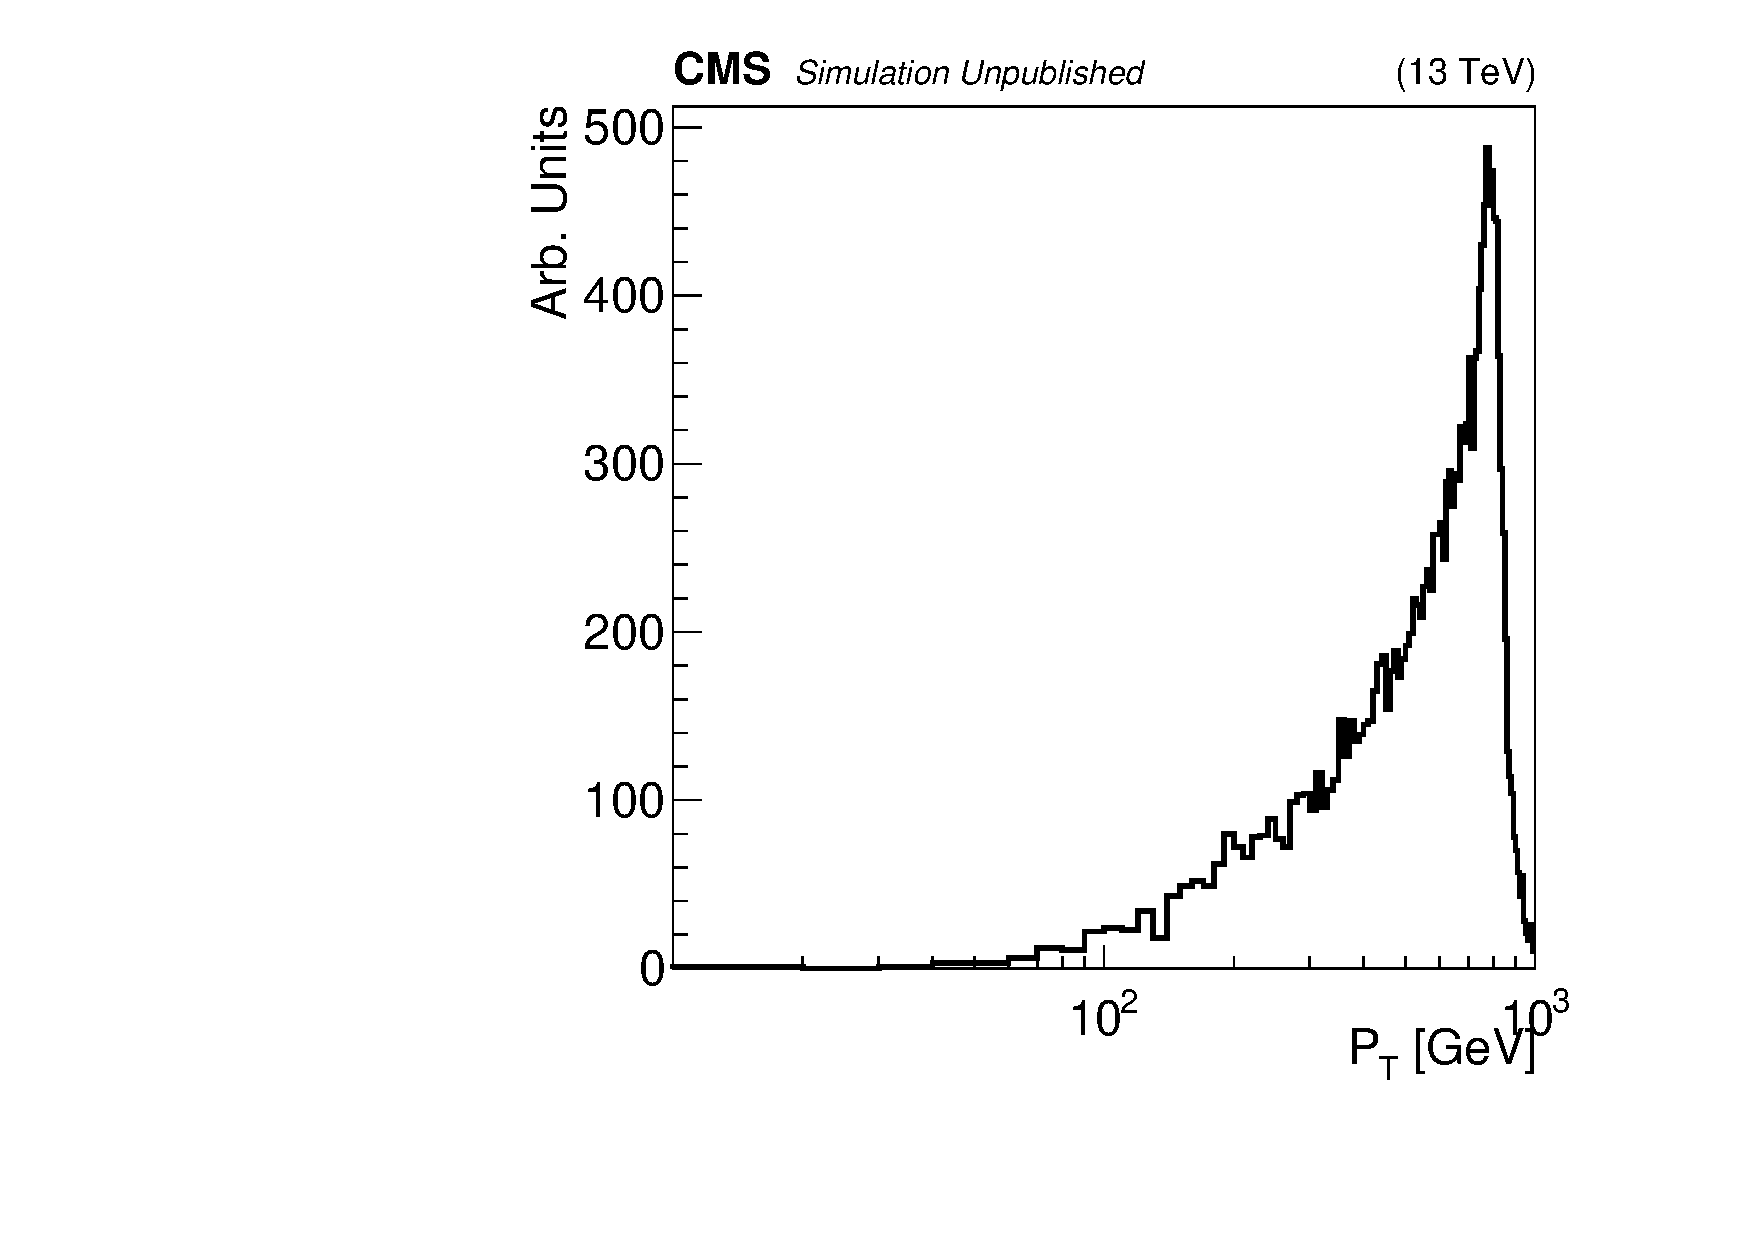
\includegraphics[width=0.65\textwidth]{figures/ptMatchedRecoEleFromWr_mwr2200_mnu1100.pdf}
	}
	\subfigure{
		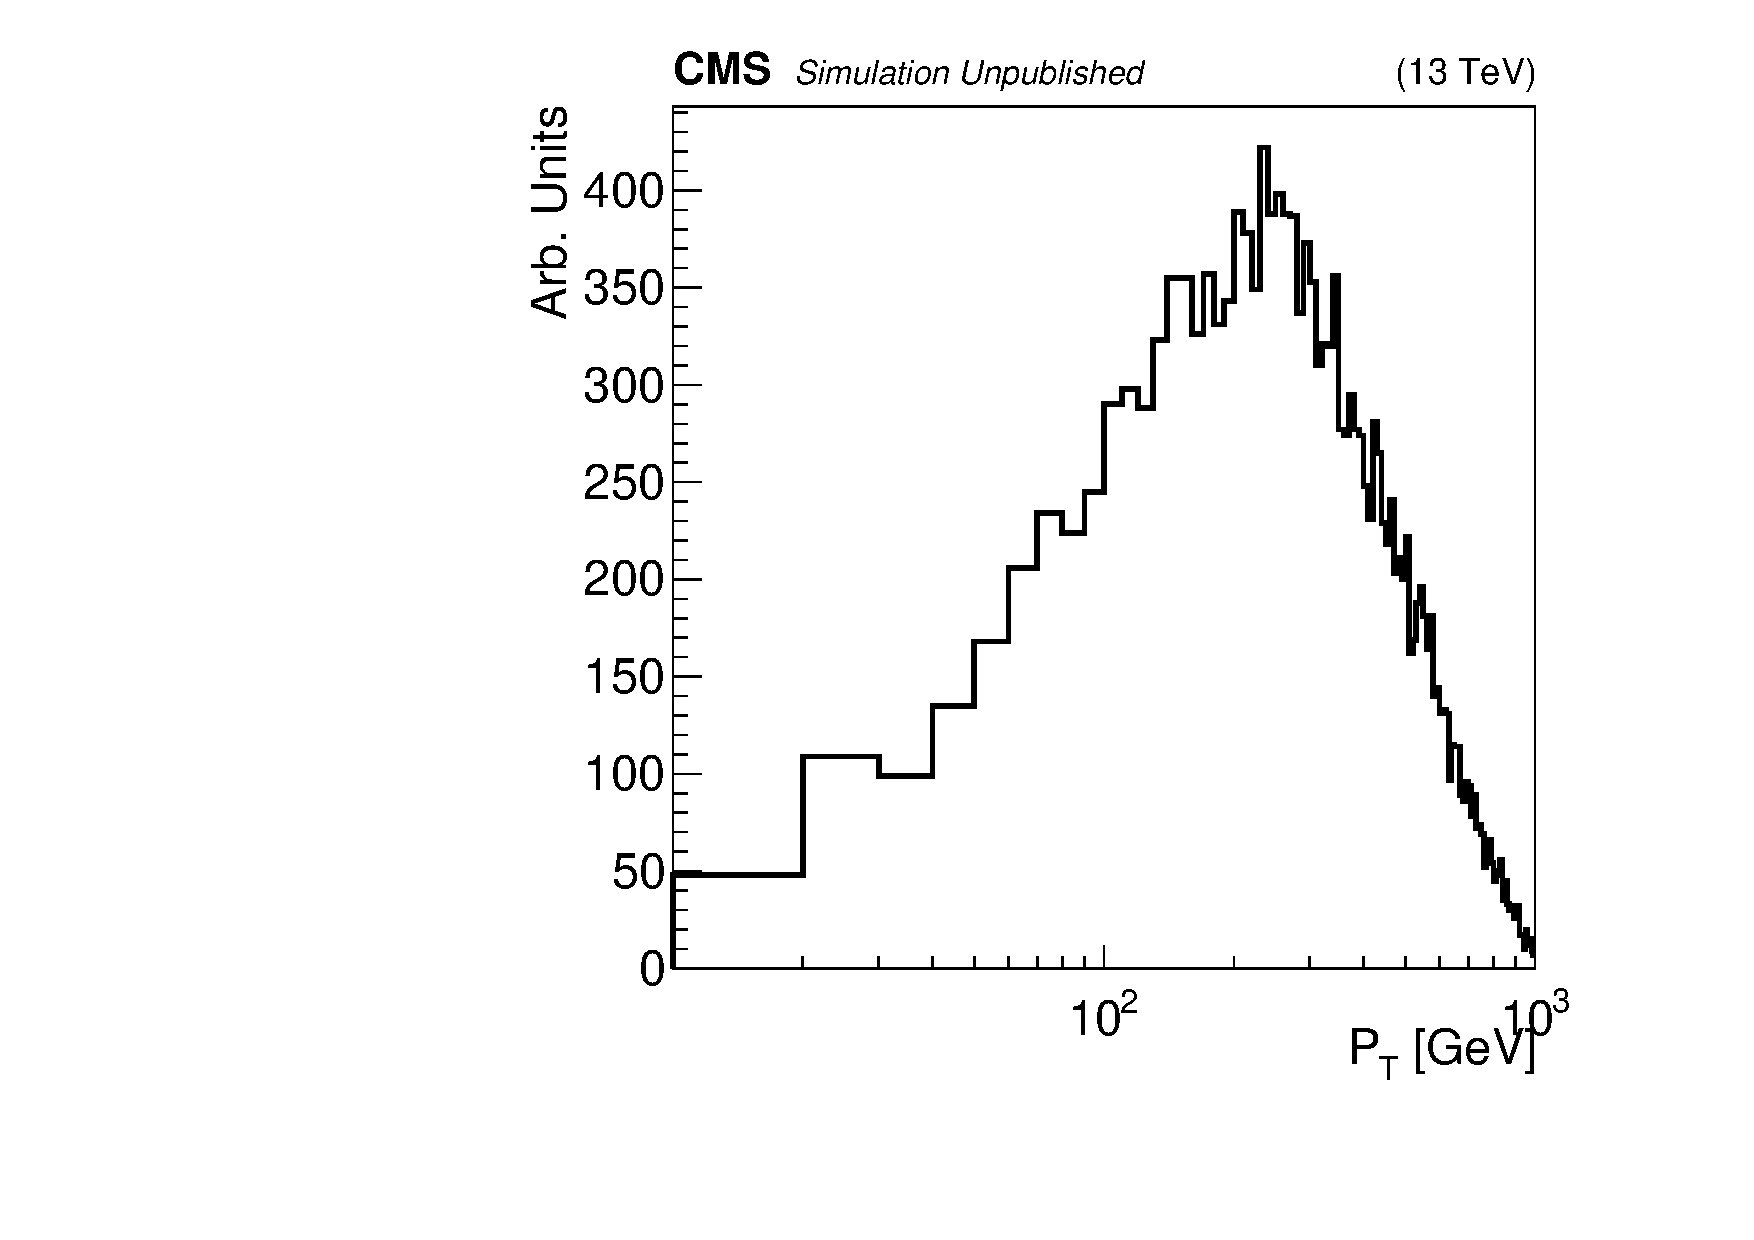
\includegraphics[width=0.65\textwidth]{figures/ptMatchedRecoEleFromNu_mwr2200_mnu1100.pdf}
	}
	\label{fig:wrLeptonPts}
	\caption{The $\pt$ distribution of the reconstructed electron produced by the \WR (\nul) decay is shown on the top (bottom) for 
		simulated $\WR \rightarrow eejj$ events with $\mWR = 2.2 \TeV$ and $\mnul = 1.1 \TeV$.}
\end{figure}

\begin{figure}[btp]
	\centering
	\subfigure{
		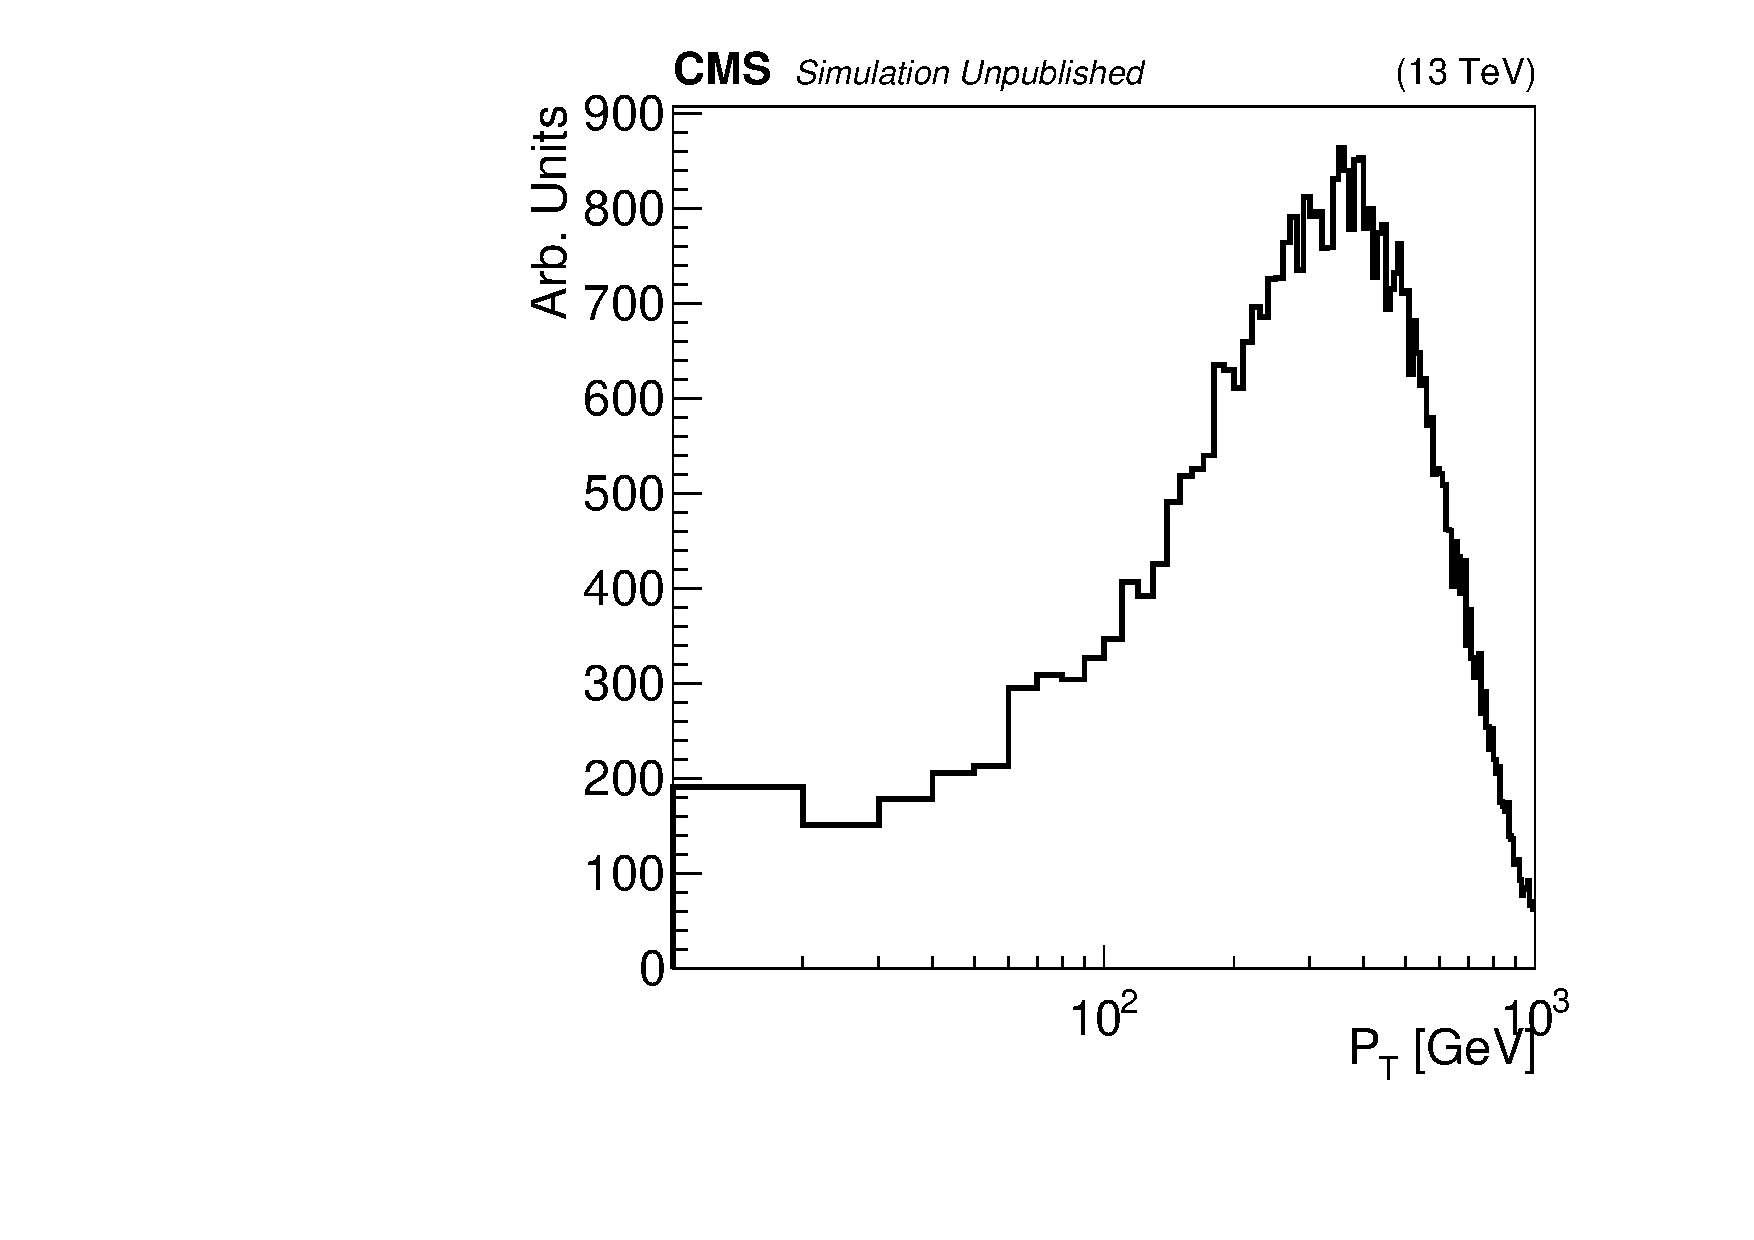
\includegraphics[width=0.65\textwidth]{figures/ptMatchedRecoJetOne_mwr2200_mnu1100.pdf}
	}
	\subfigure{
		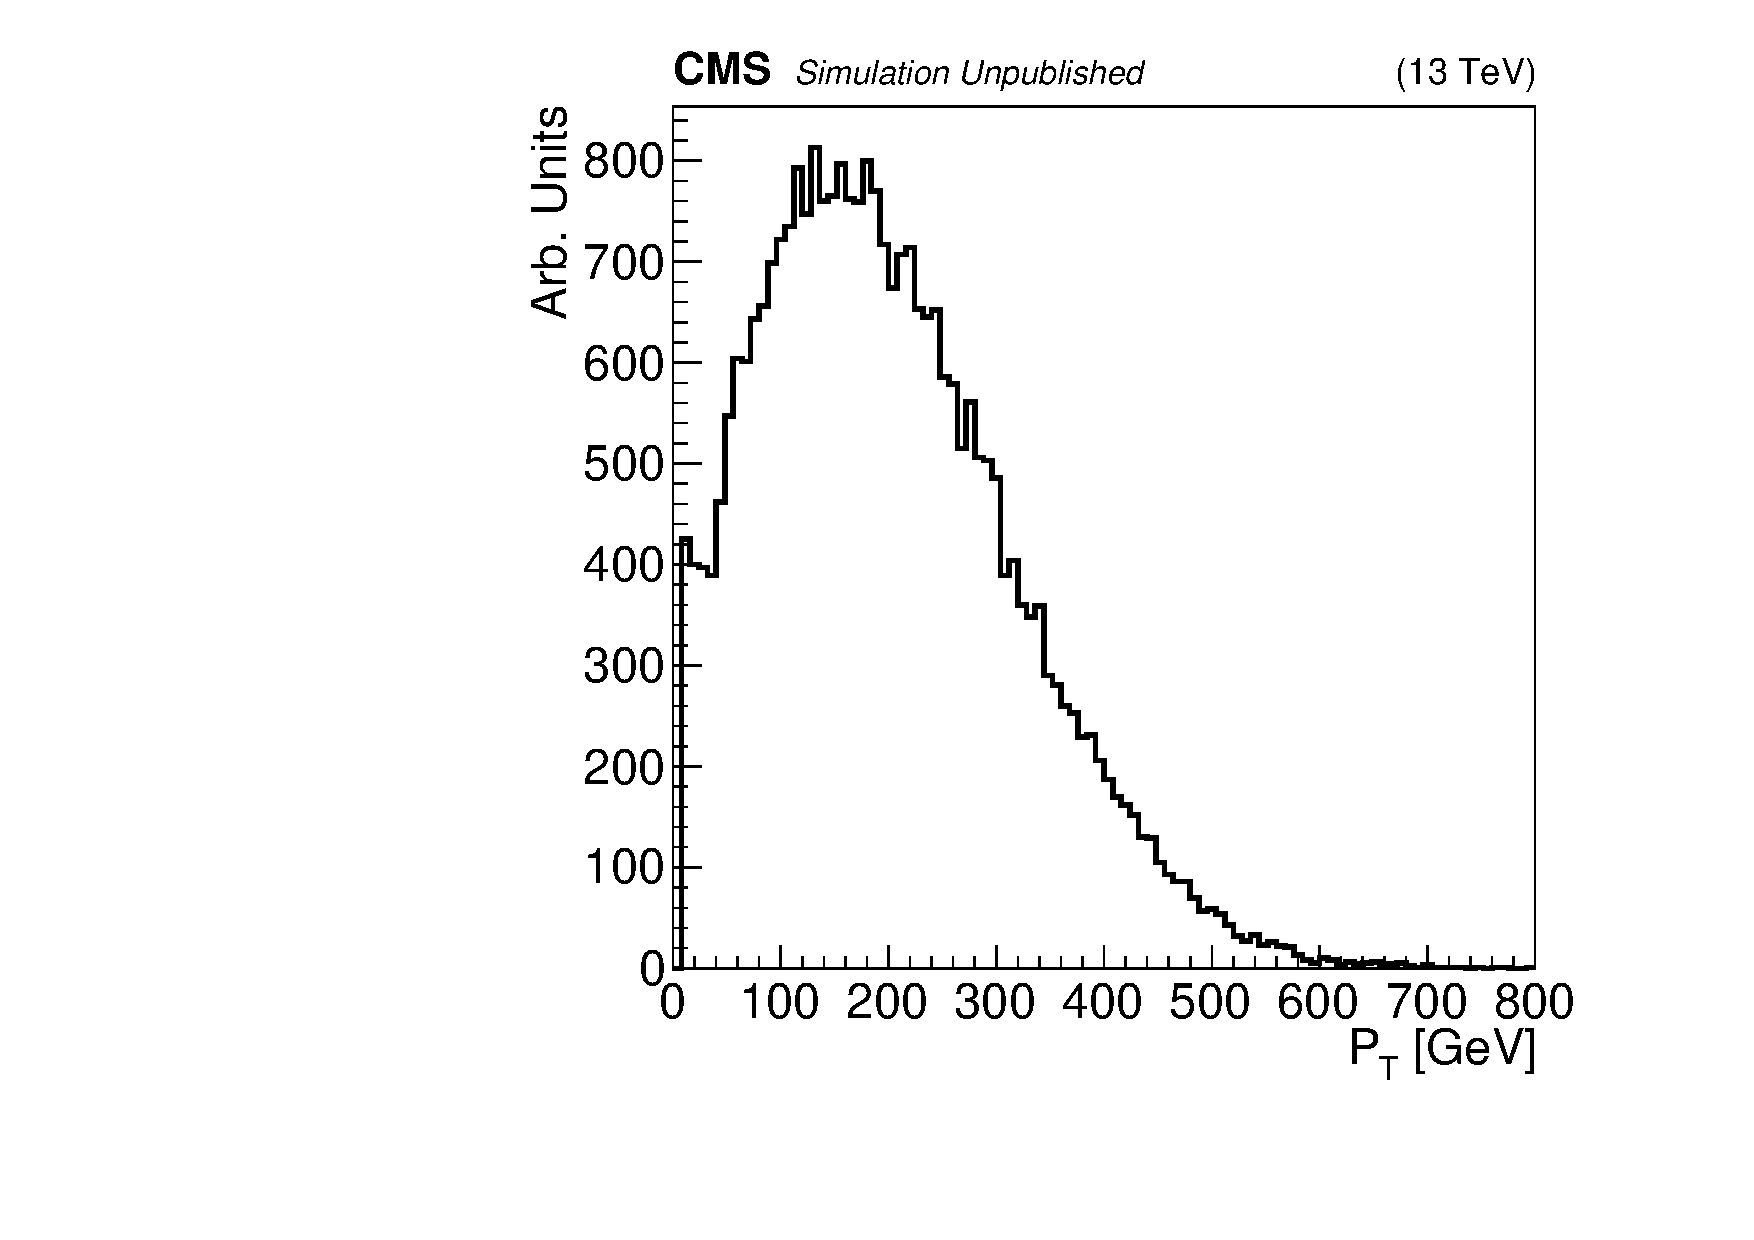
\includegraphics[width=0.65\textwidth]{figures/ptMatchedRecoJetTwo_mwr2200_mnu1100.pdf}
	}
	\label{fig:wrJetPts}
	\caption{The $\pt$ distributions of the reconstructed jets produced by the \nul decay are shown for 
		simulated $\WR \rightarrow eejj$ events with $\mWR = 2.2 \TeV$ and $\mnul = 1.1 \TeV$.}
\end{figure}

\begin{figure}[btp]
	\centering
	\subfigure{
		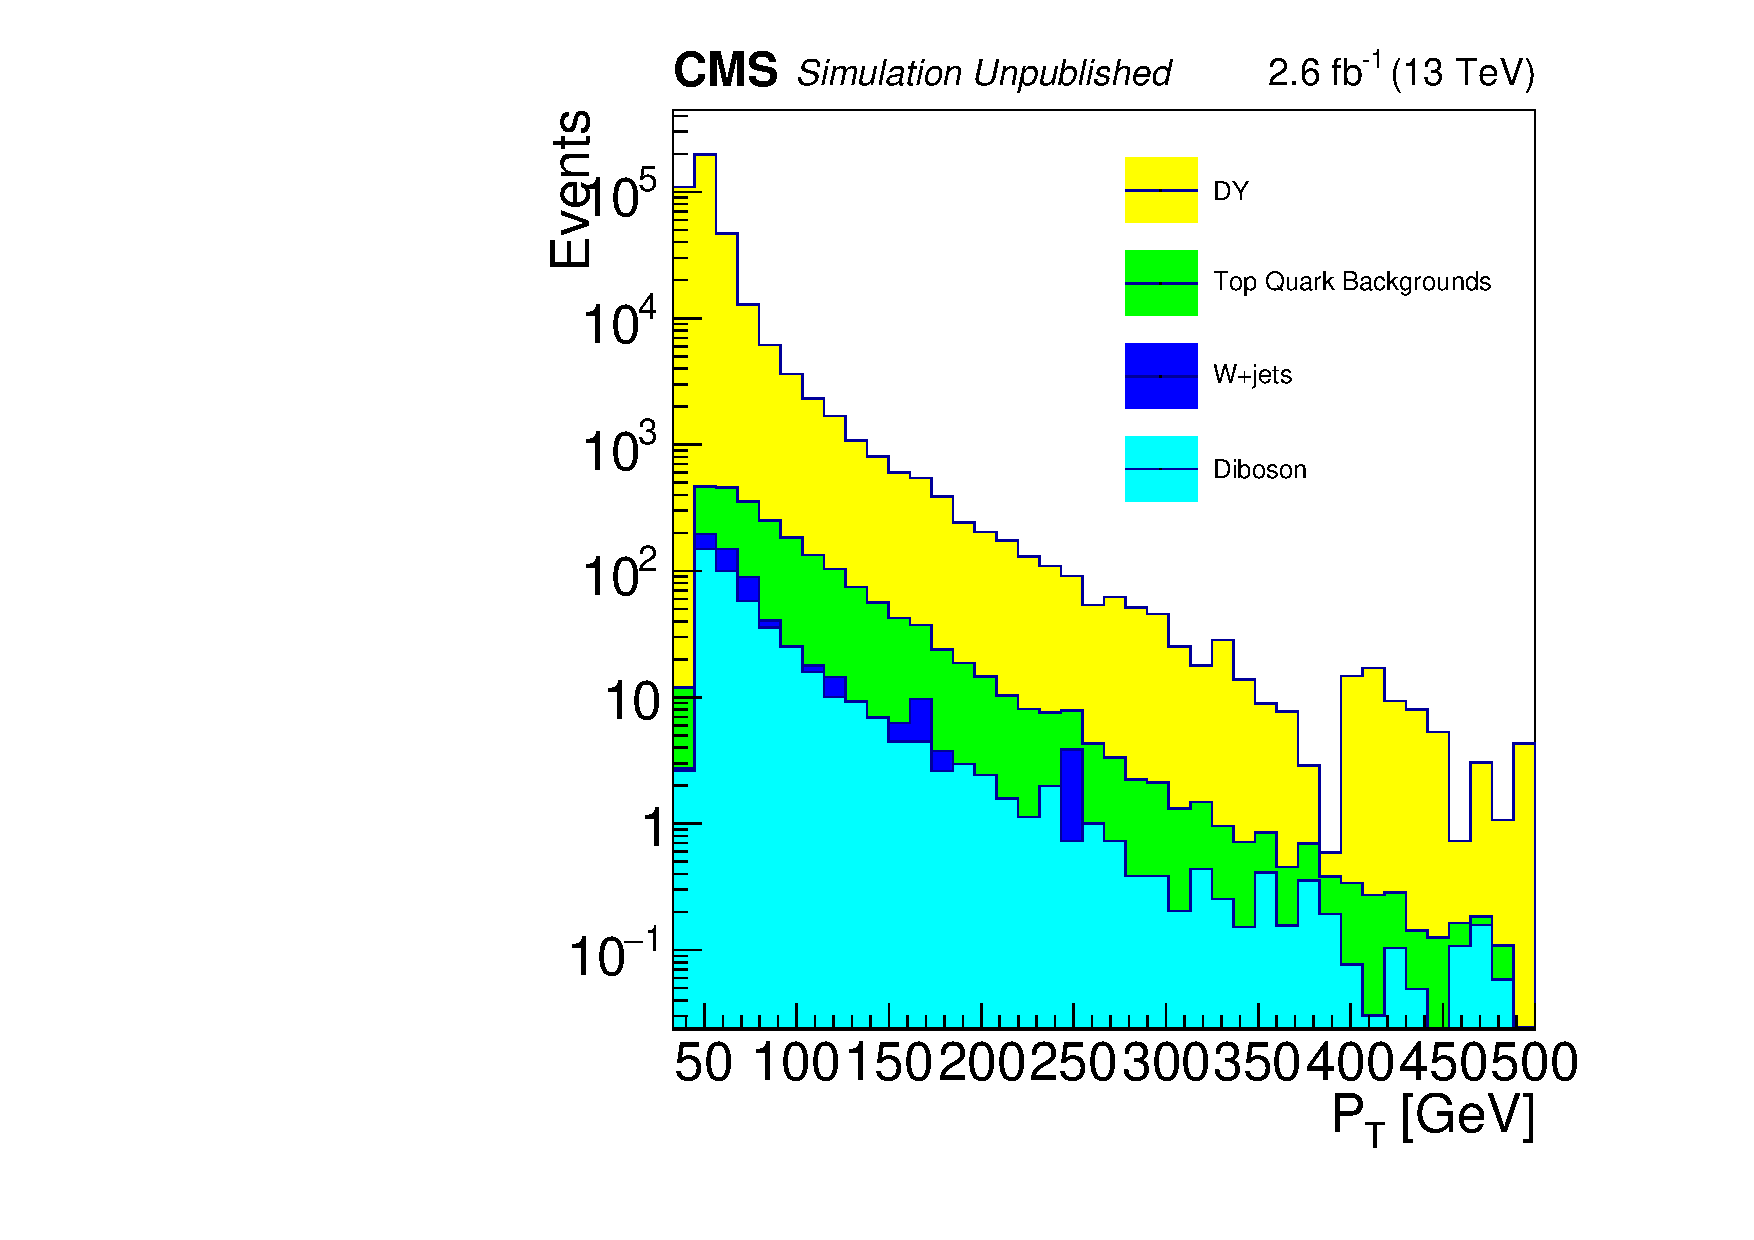
\includegraphics[width=0.65\textwidth]{figures/l1_pt_LooseSelection_TwoLeptsAndJets_EEChannelBkgndMC_log.pdf}
	}
	\subfigure{
		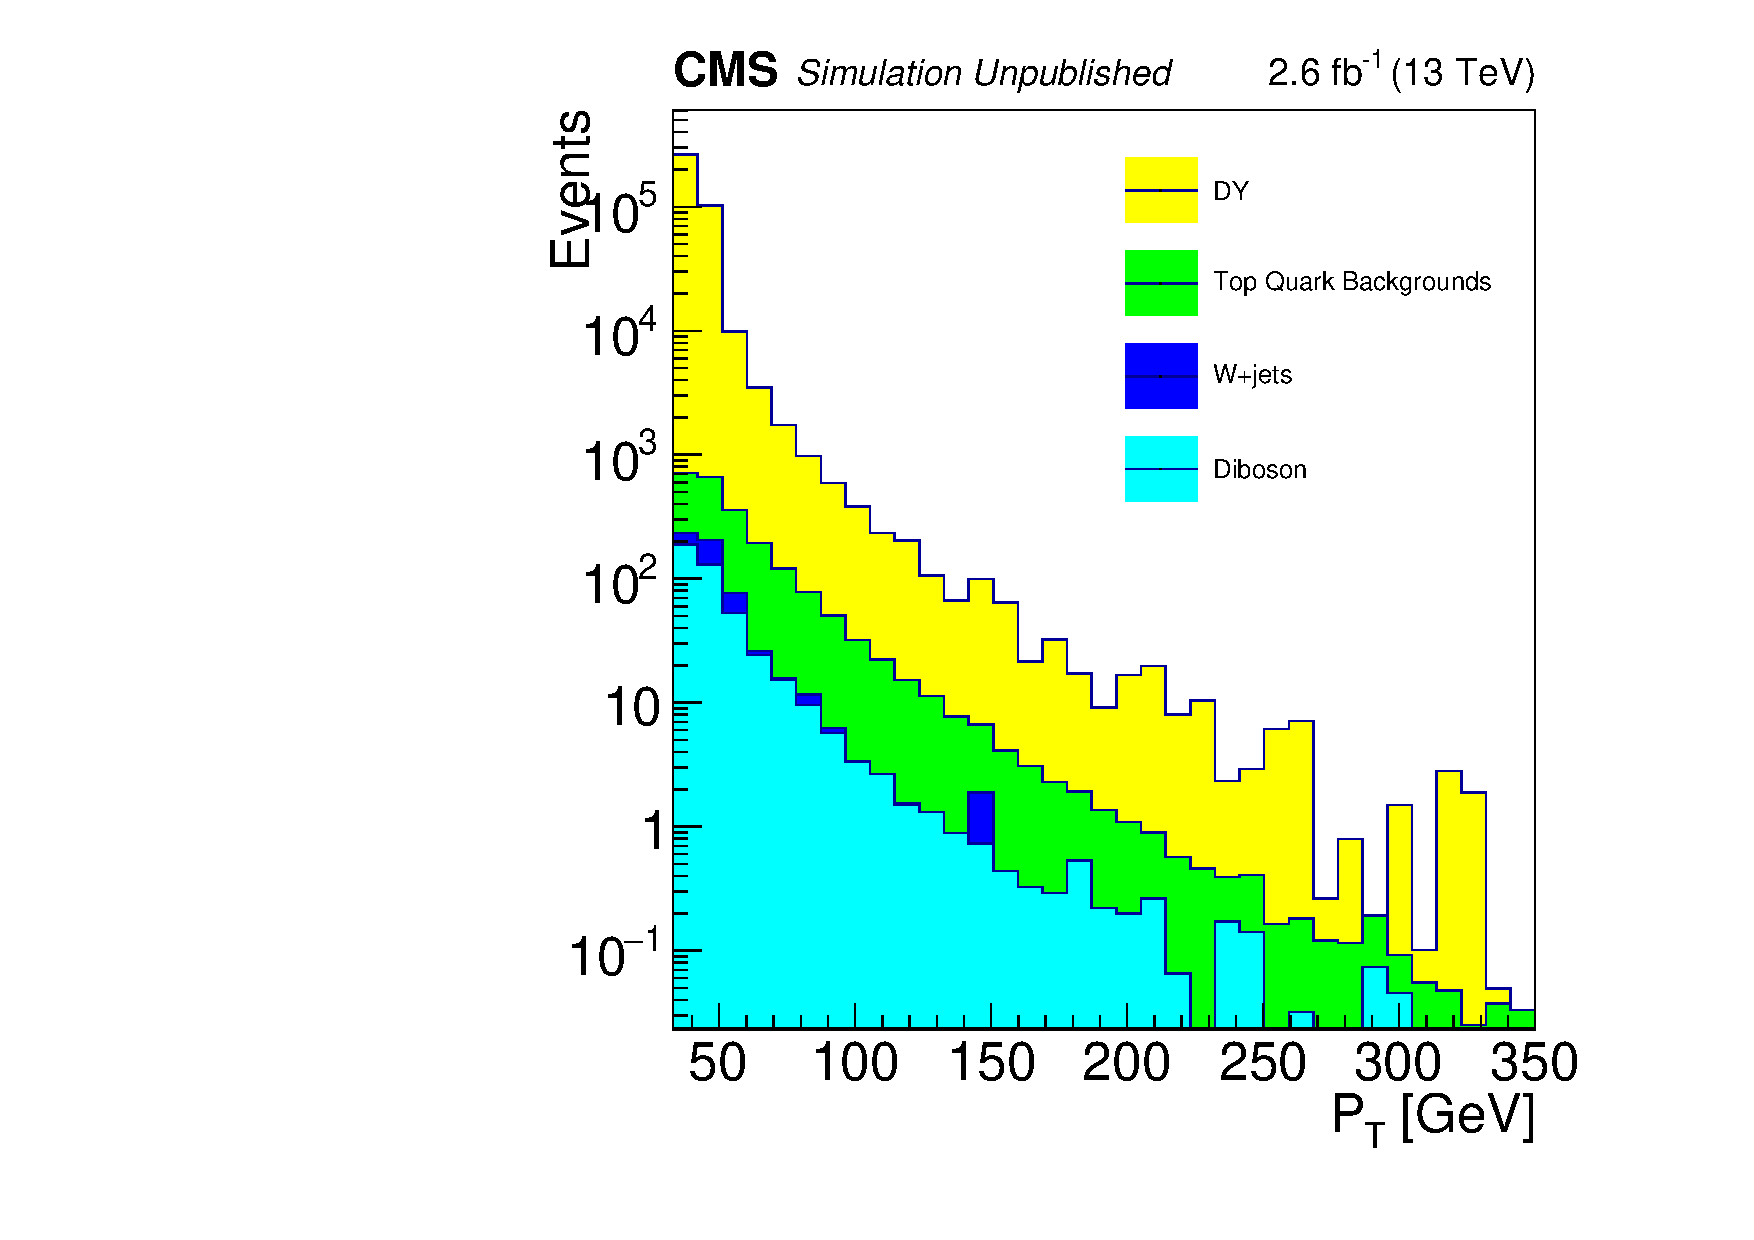
\includegraphics[width=0.65\textwidth]{figures/l2_pt_LooseSelection_TwoLeptsAndJets_EEChannelBkgndMC_log.pdf}
	}
	\label{fig:bkgLeptonPts}
	\caption{The $\pt$ distribution of the leading (subleading) electron reconstructed with $|\eta| < 2.4$ in simulated ST background events 
		with two reconstructed jets is shown on the top (bottom).  Both electrons are required to have $\pt > 33$ $\GeV$.}
\end{figure}

\begin{figure}[btp]
	\centering
	\subfigure{
		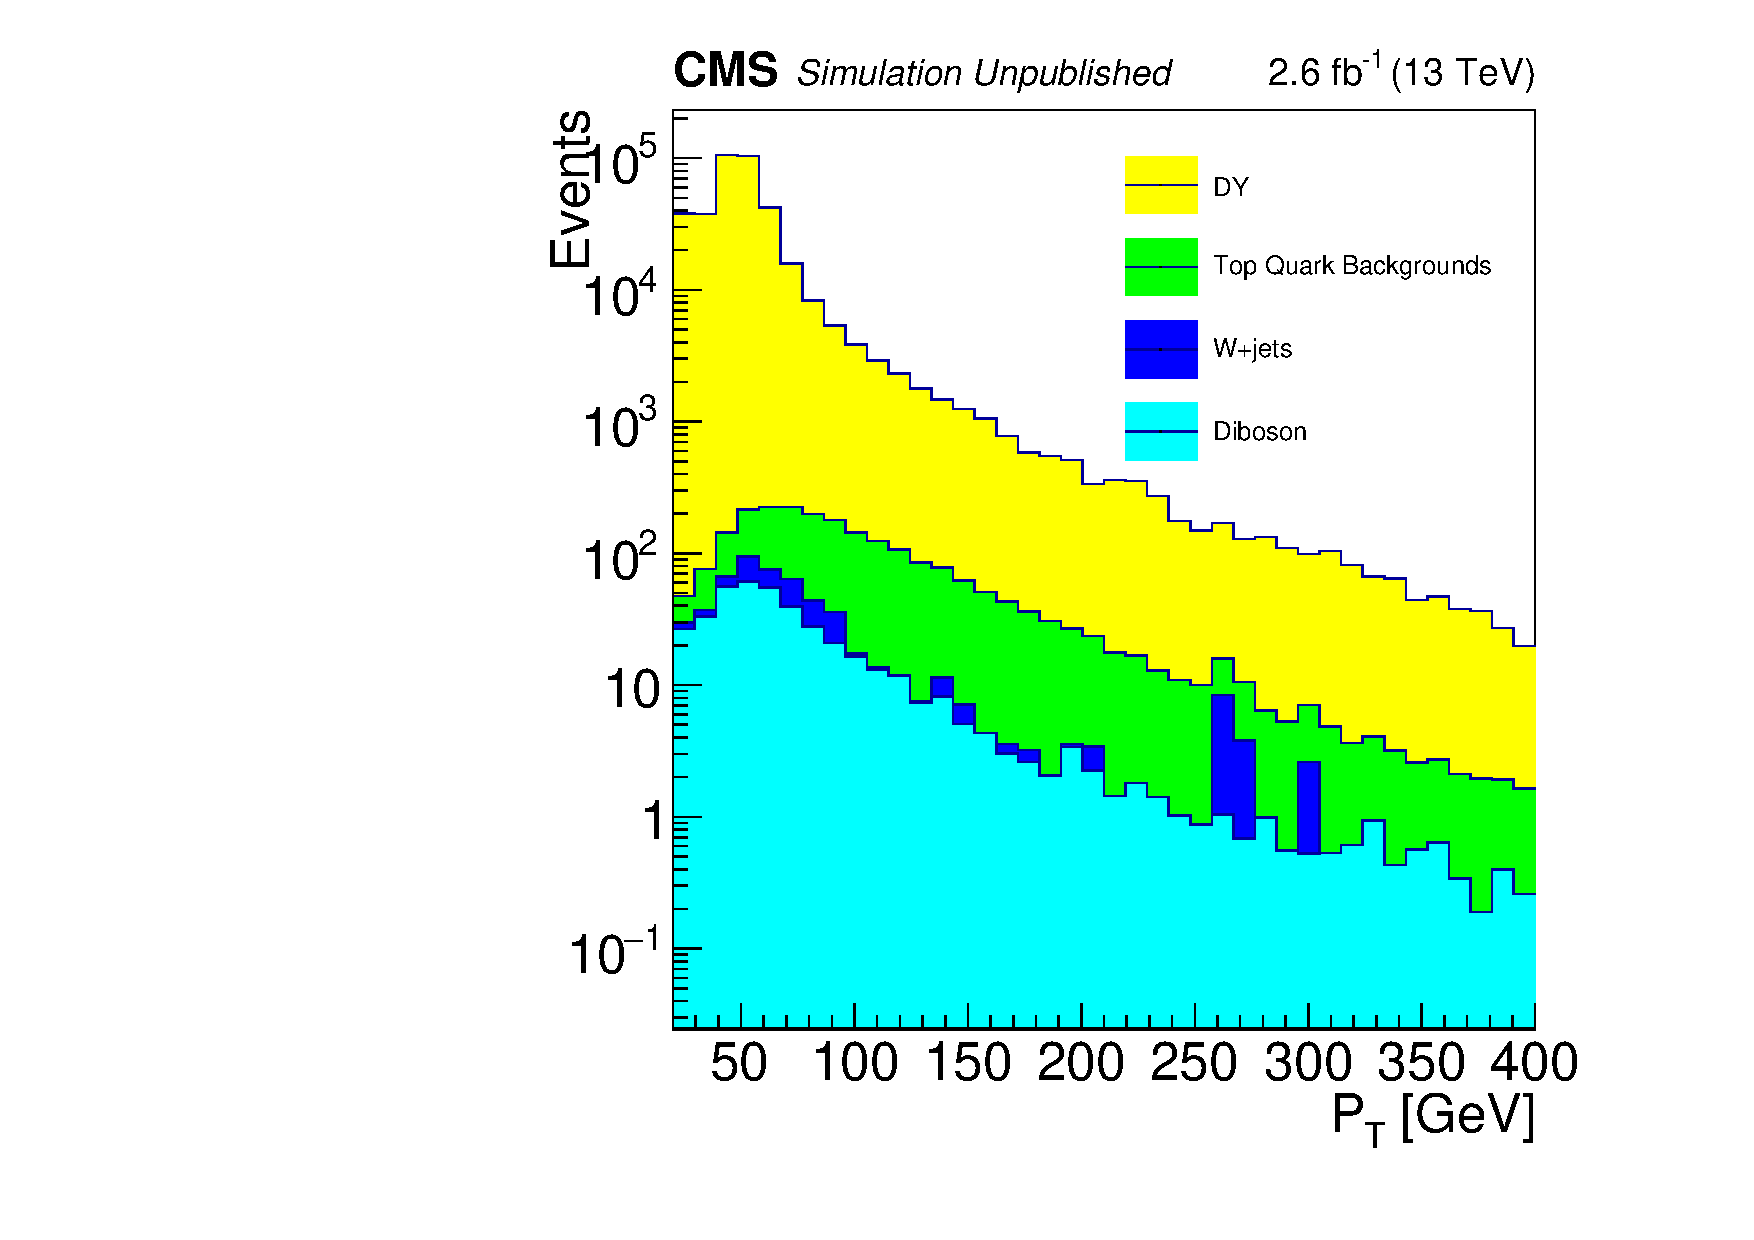
\includegraphics[width=0.65\textwidth]{figures/j1_pt_LooseSelection_TwoLeptsAndJets_EEChannelBkgndMC_log.pdf}
	}
	\subfigure{
		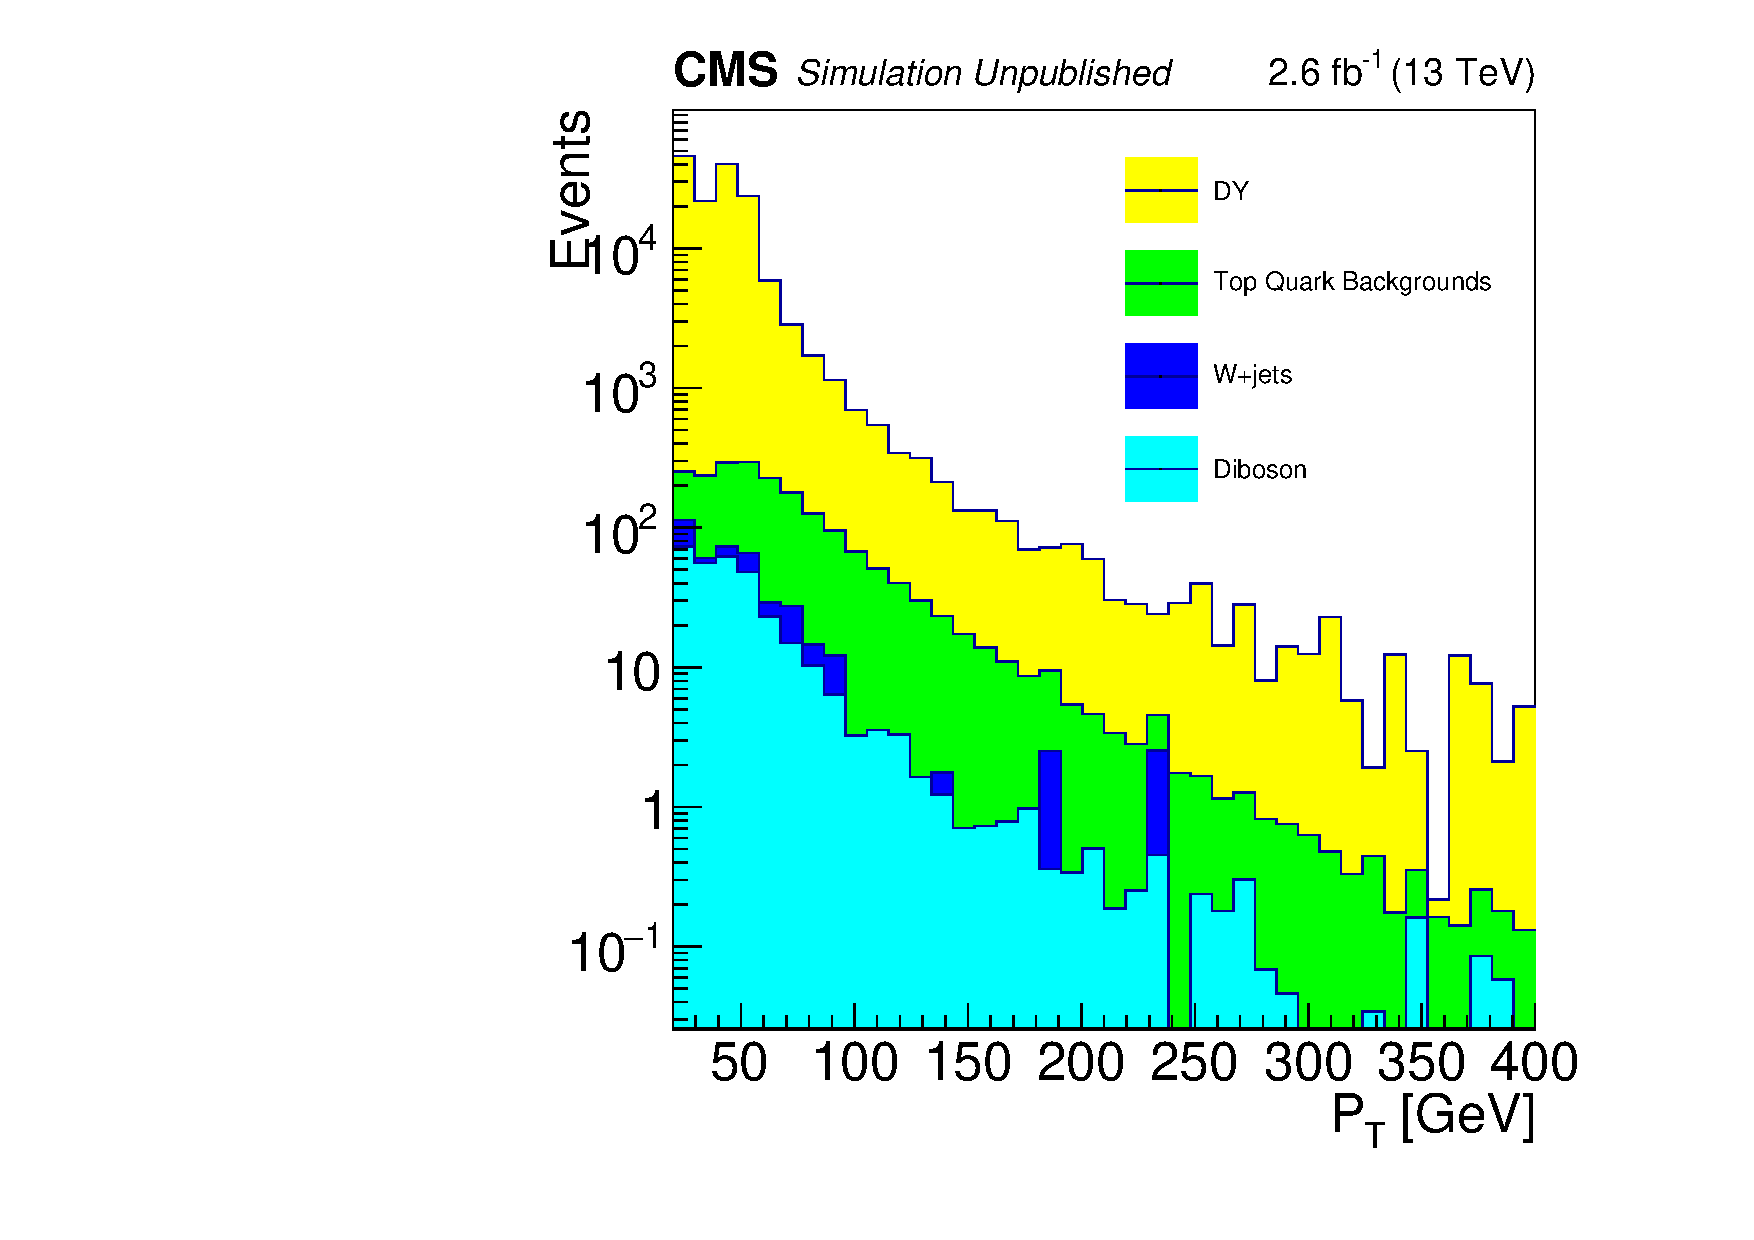
\includegraphics[width=0.65\textwidth]{figures/j2_pt_LooseSelection_TwoLeptsAndJets_EEChannelBkgndMC_log.pdf}
	}
	\label{fig:bkgJetPts}
	\caption{The $\pt$ distribution of the leading (subleading) jet reconstructed with $|\eta| < 2.4$ in simulated ST background events with 
		two reconstructed electrons is shown on the top (bottom).  Both electrons are required to have $\pt > 33$ $\GeV$.}
\end{figure}

\begin{table}[h]
	\caption{The fraction of simulated $\WR \rightarrow eejj$ events with dilepton mass $\Mll > 200$ \GeV. ($\mnul = \frac{1}{2}\mWR$)}
	\label{tab:wrMll}
	\centering
	\begin{tabular}{c|c}
		\mWR (\TeV) & Fraction of events with high \Mll (\%) \\  \hline
		1.0 &  88.  \\
		2.0 &  98.  \\
		3.0 &  99.  \\ \hline
	\end{tabular}
\end{table}

%\begin{figure}[btp]
%	\centering
%	
\includegraphics[width=0.65\textwidth]{figures/missingImage.png}
%	\label{fig:wrSigMll}
%	\caption{The dilepton mass $\Mll$ distribution for $\WR \rightarrow \mu\mu jj$ events with 
%	$\mWR = 2.0 \TeV$ and $\mnul = 1.0 \TeV$.}
%\end{figure}

%\begin{figure}[btp]
%	\centering
%	\subfigure{
%		
\includegraphics[width=0.65\textwidth]{figures/missingImage.png}
%	}
%	\subfigure{
%		
\includegraphics[width=0.65\textwidth]{figures/missingImage.png}
%	}
%	\label{fig:wrLeadLeptJetSeparation}
%	\caption{The $\Delta R(\ell,j)$ separation between the leading reconstructed muon and leading (sub-leading) reconstructed jet 
%		is shown on the top (bottom) for $\WR \rightarrow eejj$ events with $\mWR = 2.0 \TeV$ and $\mnul = 1.0 \TeV$.}
%\end{figure}
%
%\begin{figure}[btp]
%	\centering
%	\subfigure{
%		
\includegraphics[width=0.65\textwidth]{figures/missingImage.png}
%	}
%	\subfigure{
%		
\includegraphics[width=0.65\textwidth]{figures/missingImage.png}
%	}
%	\label{fig:wrSubleadLeptJetSeparation}
%	\caption{The $\Delta R(\ell,j)$ separation between the sub-leading reconstructed muon and leading (sub-leading) reconstructed jet 
%		is shown on the top (bottom) for $\WR \rightarrow eejj$ events with $\mWR = 2.0 \TeV$ and $\mnul = 1.0 \TeV$.}
%\end{figure}


\section{Monte Carlo}
\label{sec:MC}
Monte Carlo (\MC) simulations were used to predict ST backgrounds, and to study lepton and jet kinematics 
in $\WR \rightarrow \ell\ell jj$ events.  ST backgrounds were processes like $Z+jets \rightarrow \ell\ell+jets$ 
and $W+jets \rightarrow \ell\nu+jets$ that produced events where 2 leptons and 2 jets were reconstructed 
and passed all selections.  \MC simulations of ST backgrounds and \WR signals were produced using the 
following procedure:

\begin{itemize}
	\item In \textbf{step 1} a dedicated \MC generator was used to simulate the interaction between two protons 
		colliding in a vacuum, and the particles produced by the interaction.
	\item In \textbf{step 2} the effect of multiple pp interactions occurring in the same collision was simulated, 
		and GEANT4 \cite{geant4} was used to simulate interactions between particles and detector materials, 
		and the detector response to particles.
	\item In \textbf{step 3}the simulated detector response was used to simulate the Level-1 and High Level 
		trigger decisions, and to reconstruct particles and interaction vertices using the same reconstruction 
		algorithms used in data.
\end{itemize}

In step 1 the \MC generator also simulated the decay of unstable particles, and hadronized partons into jets.  
Before starting step 2, an independent \MC simulation of minimum bias collisions was produced using step 1.  
Then, for every event $i$ simulated in step 2, a random integer $X$ representing the number of pileup interactions 
was pulled from a Poisson distribution with mean twelve\footnote{When 2015 \MC simulations began, the average expected 
pileup per event was 12}.  $X$ simulated minimum bias events were added to the primary event $i$ before starting GEANT4 
simulations.  In step 3, trigger decisions were saved but were not used to exclude events from reconstruction.  This 
3 step procedure was used to simulate the ST backgrounds and \WR signals listed in Table \ref{tab:centrallyProducedMC}.

The distribution of the number of pileup interactions per event was identical for all simulated datasets, and 
differed in shape from the distribution found in data.  This shape difference was resolved by applying a pileup 
dependent weight to every simulated event.

\begin{table}[bt]
\caption{The simulated datasets used to study ST backgrounds and the \WR signal.  The "Size" of a dataset is equal 
	to the number of simulated events divided by the 13 $\TeV$ cross section $\times$ branching fraction of the process.}
\label{tab:centrallyProducedMC}

\centering
\resizebox{\textwidth}{!}{
	\begin{tabular}{ |c|c|c|c| } 
	\hline
	Dataset         & Step 1 Generator & cross section (pb) & Size (fb$^{-1}$)   \\
		\hline
		Inclusive DY+jets, $DY \rightarrow ll$ & \MADGRAPH   & 5991    & 1.51 \\ \hline
		DY+jets HT 100-200, $DY \rightarrow ll$ & \MADGRAPH   & 181.3    & 15.0 \\ \hline
		DY+jets HT 200-400, $DY \rightarrow ll$ & \MADGRAPH   & 50.42    & 19.3 \\ \hline
		DY+jets HT 400-600, $DY \rightarrow ll$ & \MADGRAPH   & 6.984    & 153. \\ \hline
		DY+jets HT $>$ 600, $DY \rightarrow ll$ & \MADGRAPH   & 2.704    & 369. \\ \hline
		\ttbar+jets $\rightarrow ll$+jets & \MADGRAPH  & 85.67    & 286. \\ \hline
		single t $\rightarrow$ leptons+jets  & \POWHEG & 80.95 & 20.8 \\ \hline
		single $\bar{t}$ $\rightarrow$ leptons+jets & \POWHEG & 136.0 & 24.3 \\ \hline
		$\bar{t}$+W $\rightarrow$ all   & \POWHEG & 35.85 & 27.6 \\ \hline
		t+W $\rightarrow$ all   & \POWHEG & 35.85 & 27.8 \\ \hline
		WW $\rightarrow$ all  & \PYTHIA & 113.8   & 8.73   \\ \hline
		ZZ $\rightarrow$ all  & \PYTHIA & 10.15   & 98.2   \\ \hline
		WZ $\rightarrow$ all  & \PYTHIA & 23.4   & 41.8   \\ \hline
		W+jets $\rightarrow l\nu$+jets & \MADGRAPH & 50270   & 1.44 \\ \hline
		$\WR \rightarrow l\nul \rightarrow lljj$  & \PYTHIA & 1$\times 10^{-5}$ - 4.3 & 5$\times 10^{6}$ - 11.6   \\ \hline
		\end{tabular}
}
\end{table}

In step 1 different \MC generators were used based on the characteristics of the process being simulated.  The 
\MADGRAPH \cite{madgraph} generator simulated all leading order Feynman diagrams of an interaction with up to 4 
additional radiated partons, which produced additional jets.  The effect of additional jets on the number of 
events passing the selections described in Chapter \ref{sec:signalAndBkgndFeatures} was significant 
only in high cross section ST backgrounds - $DY \rightarrow \ell\ell$, $t\bar{t} \rightarrow \ell\ell jj$, and 
$W \rightarrow \ell\nu$.  Although all ST background simulations would produce more events passing the 
selections if additional radiated partons were simulated, other ST backgrounds had 
cross sections $\times$ branching fractions to $\ell\ell jj$ final states that were much lower than those of $DY$, 
$\ttbar$, and $W \rightarrow \ell\nu$; the contribution of other backgrounds to the total background after selections 
was negligible, regardless of additional parton radiation.  Therefore, \MADGRAPH was used to simulate the $DY$, $\ttbar$, and 
$W \rightarrow \ell\nu$ backgrounds with additional radiation partons, but was not used to simulate other backgrounds 
for two reasons: the way \MADGRAPH simulated additional parton radiation made it one of the most time consuming generators, and 
it only simulated interactions at leading order in the electroweak and strong coupling constants.  The cross sections 
$\times$ branching fractions of other top and $\bar{t}$ quark backgrounds, like $\bar{t}$+W, to $\ell\ell jj$ final 
states were sensitive to next-to-leading order electroweak corrections, so the next-to-leading order \POWHEG \cite{powheg} generator 
was used to simulate these backgrounds.  The cross sections $\times$ branching fractions of diboson (WW, WZ, ZZ) backgrounds 
to $\ell\ell jj$ final states were so low that the next-to-leading order electroweak corrections were irrelevant.  
To save simulation time and computing resources, the leading order \PYTHIA \cite{pythia8,Sjostrand:2006za} generator 
was used to simulate the diboson backgrounds.  In all simulations, \PYTHIA with the NNPDF23 PDF set \cite{nnpdf} 
was also used to hadronize partons into jets.

The \WR signal model assumes negligible mixing between left- and right-handed fermions, so the next-to-leading 
order electroweak corrections have a negligible impact on the signal.  \PYTHIA was used to simulate the 
\WR signal using the NNPDF23 PDF set.  A large range of \mWR values were studied by generating datasets with \mWR 
stepping from 0.8 to 6 $\TeV$ in increments of 0.2 $\TeV$, and requiring $\mnul = \frac{1}{2}\mWR$.

Additional $\WR \rightarrow \ell\ell jj$ datasets were produced with \PYTHIA, and used in the situation when no \WR 
signal was found.  Events were simulated only through step 1, and using the same \PYTHIA configuration used in the 
full 3 step simulation.  Datasets were produced with \mWR stepping from 0.8 to 4.0 $\TeV$ in increments of 0.1 $\TeV$.  
At each \mWR, several datasets were produced with $0.025 \leq \mnul < \mWR$ $\TeV$.  If no \WR signal was found, these 
datasets were used to test observations from data against predictions made by different $(\mWR, \mnul \neq \frac{1}{2}\mWR)$ 
hypotheses, and set \mWR and \mnul exclusion limits.


\section{Online Event Selection}
\label{sec:triggers}
Evidence of a \WR and \nul was searched for in events selected during collisions by lepton triggers.  The $ee$-channel 
search used a double electron HLT algorithm, and the $\mu\mu$-channel search used a single muon HLT algorithm.

In the $ee$-channel, events were first selected by Level-1 triggers that required one ECAL supercluster (SC) 
with $\Et > 40 \GeV$, or two non-overlapping SCs: one with $\Et > 22$ $\GeV$, the other with $\Et > 10$ $\GeV$.  
Events that passed the Level-1 selection were reconstructed offline if they passed the following double electron 
HLT selections:

\begin{itemize}
	\item Two non-overlapping SCs were detected with $\Et > 33$ $\GeV$.
	\item For each SC:
	\begin{itemize}
		\item The ratio of hadronic energy in the HCAL tower behind the SC to the SC energy was $< 0.15$ in the barrel, and $< 0.1$ in the endcap.
		\item Ninety percent of the SC energy was measured in an $(\eta, \phi)$ region that was two crystals wide in $\eta$.
		\item If the SC was in the barrel, a reconstructed track with hits in at least two pixel tracker layers extrapolated to the SC 
			centroid along the beam axis within $2.3$ cm, and extrapolated to the SC centroid in $(\eta, \phi)$ within the $(\eta, \phi)$ 
			area of one ECAL crystal.
	\end{itemize}
\end{itemize}

In the $\mu\mu$-channel, events were first selected by a Level-1 trigger that required a track in at least one muon DT or 
CSC detector with $\pt > 16$ $\GeV$.  Events that passed the Level-1 selection were reconstructed offline if they 
passed the following single muon HLT selections:

\begin{itemize}
	\item A track reconstructed in the silicon tracker with $\pt > 50$ $\GeV$ and $|\eta| < 2.4$ was geometrically matched to 
		the muon detector hits that passed the L1 trigger.  Considering this set of muon detector hits and the matching reconstructed 
		track:
	\begin{itemize}
		\item A curve representing the muon trajectory through CMS was fitted to the reconstructed track and at least 
			one muon detector hit with $\chi^{2}/nDOF < 20$.
		\item In the plane perpendicular to the beam axis, the distance between the reconstructed track origin and its 
			reconstructed vertex was $< 1$ mm.
	\end{itemize}
\end{itemize}

%add this to the background estimation chapter
%A second set of $\mu\mu$ -channel events were used only to estimate backgrounds.  These events were first 
%selected online by a Level-1 trigger, which required $>$ 20 GeV of momentum be measured in a muon 
%DT or CSC detector.  Following the Level-1 selection, events were saved to permanent storage if the 
%following single muon High Level trigger requirements were met:
%
%\begin{itemize}
%	\item Unless noted otherwise, the same requirements were applied to muon candidates in the barrel and endcap.
%	\item A global curve representing a muon candidate was fit to a reconstructed track and at least one muon detector hit with $\chi^{2}/nDOF <$ 20.
%	\item In the $x-y$ plane, the distance between the origin of the muon track and the primary vertex was $<$ 1 \mm.
%	\item The reconstructed muon track had $p_{T} >$ 22 GeV.
%	\item In a cone of radius $\Delta R =$ 0.3 centered on the muon detector energy cluster ($\thicksim$900 ECAL crystals, $\thicksim$35 HCAL towers in the cone):
%	\begin{itemize}
%		\item The total ECAL energy in the cone is small compared to the muon cluster energy, $\frac{E_{ECAL}}{E_{\mu}} < 0.11$ in the barrel, $< 0.08$ in the endcap.
%		\item The total HCAL energy in the cone is small compared to the muon cluster energy, $\frac{E_{HCAL}}{E_{\mu}} < 0.21$ in the barrel, $< 0.22$ in the endcap.
%		\item The sum $p_{T,other}$ of all tracks in the cone excluding the muon track is small compared to the muon track $p_{T,\mu}$, 
%			$\frac{p_{T,other}}{p_{T,\mu}} < 0.09$ in the barrel and endcap.
%	\end{itemize}
%\end{itemize}

%add this to the background estimation chapter
%As stated earlier, it is assumed that the $\WR$ decay cannot violate lepton 
%flavor conservation.  Therefore, evidence of a \WR and \nul was not searched for in 
%events with the $e\mu jj$ final state.  However, events in the $e\mu$ -channel 
%($e\mu jj$ final state) were used to estimate top quark backgrounds using a procedure described later.  The $e\mu$ 
%-channel events were selected by a Level-1 trigger that required a track in one 
%muon DT or CSC detector with $\pt > 16$ $\GeV$.  Events that passed the L1 selection were reconstructed if 
%they passed the following electron-muon HLT selections:
%
%\begin{itemize}
%	\item A track reconstructed in the silicon tracker with $\pt > 30$ $\GeV$ was geometrically matched to 
%		the muon detector hits that passed the L1 trigger.
%	\item A curve, representing the muon trajectory through CMS, was fitted to the silicon tracker track and 
%		at least one muon detector hit with $\chi^{2}/nDOF < 20$.
%	\item The distance in the $x-y$ plane between the origin of the silicon tracker track and its 
%		reconstructed vertex was $< 1$ \mm.
%	\item One ECAL SC was detected with energy $>$ 30 GeV.
%	\item For the SC:
%	\begin{itemize}
%		\item The ratio of hadronic energy in the HCAL tower behind the SC to the SC energy was $< 0.15$ in the barrel, and $< 0.1$ in the endcap.
%		\item Ninety percent of the SC energy was measured in an $(\eta, \phi)$ region that is two crystals wide in $\eta$.
%		\item For SCs in the barrel, a reconstructed track with hits in at least two pixel tracker layers extrapolated to the 
%			$z_{SC}$ SC center within 2.3 \cm, and the $(\eta_{SC}, \phi_{SC})$ SC center within the $(\eta, \phi)$ area of one ECAL crystal.
%	\end{itemize}
%\end{itemize}

Simulated events used in either channel were required to pass the appropriate trigger.


\section{Offline Muon Selection}
\label{sec:muonSelection}
The energies of reconstructed muons in data and simulations were corrected before applying any selections.  
The muon energy corrections were derived by comparing muon kinematic variables in $Z \rightarrow \mu\mu$ decays 
between data and simulated events.  The corrections were applied to resolve the difference in efficiency of 
muon $\pt$ selections between data and simulated events.

Following energy corrections, muon kinematic and identification (ID) selections were applied to select muons consistent 
with those expected from \WR decays.  Each event was required to have two muons reconstructed with 
$\pt > 53$ $\GeV$ and $|\eta| < 2.4$, and at least one of those muons was required to have $\pt > 60$ $\GeV$.  
Reducing the lower $\pt$ selection was explored, but was found to increase ST 
backgrounds without a corresponding increase in \WR signal, as shown in Table \ref{tab:lowerMuonPtCuts}.  Muons 
passing kinematic selections were filtered with the following ID selections:

\begin{itemize}
	\item Considering the muon's track reconstructed in the silicon tracker:
	\begin{itemize}
		\item The track was reconstructed from at least 1 hit in the silicon pixel detector, and at least 
			5 hits in the entire tracker.
		\item Within a cone of radius $\Delta R = 0.3$ centered on the track, the $\sum \pt$ of all other 
			reconstructed tracks was low compared to the muon $\pt$, $\frac{\sum \pt}{muon \pt} < 0.1$.
	\end{itemize}
	\item The muon was detected in at least 2 muon chambers.
	\item The fitted track representing the estimated muon trajectory through all of CMS originated at a 
		point that was within 2 (5) mm of the muon's reconstructed vertex in the $x-y$ plane ($z$ axis). 
	\item The muon momentum measurement included at least one muon chamber hit.
	\item The error on the muon momentum measurement, $\sigma(\pt)$, was less than 30\% of the muon $\pt$, 
		$\sigma(\pt)/\pt < 0.3$.
\end{itemize}

\begin{table}[h]
	\caption{Signal (S) over background (B) sensitivity, represented by S/$\sqrt{B}$, for different $\mu$ $\pt$ 
	selections.  The background is estimated from simulated \DY and t$\bar{t}$, and the signal is estimated 
	from simulated $\WR \rightarrow \mu\mu jj$ with $\mWR = 2.2 \TeV$ and $\mnul = 1.1 \TeV$.}
	\label{tab:lowerMuonPtCuts}
	\centering
	\begin{tabular}{c|c}
		$\mu$ $\pt$ threshold ($\GeV$) & S/$\sqrt{B}$ \\  \hline
		40 &  11.9  \\
		53 &  12.6  \\ \hline
	\end{tabular}
\end{table}

If an event contained more than two muons passing all kinematic and ID selections, the two highest $\pt$ muons 
were selected.

The efficiencies of muon reconstruction, trigger and ID selections differed between simulations and data, and 
the differences were corrected by applying multiplicative weights to simulated events.  Trigger 
and reconstruction+ID weights were calculated as functions of the charge and kinematic variables of selected 
muons.  The trigger weight, between 0.95 (5\% decrease) and 1.04 (4\% increase), was applied once to every 
event, and the reconstruction+ID weight, between 1.0 and 0.985 (1.5\% decrease), was applied twice to 
every event.


\section{Offline Electron Selection}
\label{sec:electronSelection}
The energies of reconstructed electrons in data and simulations were corrected before applying any selections.  Similar 
to muons, the electron energy corrections were derived by comparing electron kinematic variables in $Z \rightarrow ee$ decays 
between data and simulated events.  The corrections were applied to resolve the difference in efficiency of 
electron $\Et$ selections between data and simulated events.

Following energy corrections, electron kinematic and ID selections were applied to select electrons 
consistent with those expected from \WR decays.  Each event was required to have two electrons reconstructed 
with $\Et > 53$ $\GeV$ and $|\eta| < 2.4$, and at least one of those electrons was required to have $\Et > 60$ $\GeV$.  
Electrons passing kinematic selections were filtered with the following ID selections:

\begin{itemize}
	\item Electrons were ignored if they were reconstructed in the dead zone separating the ECAL barrel and 
		endcap detectors, $1.44 < |\eta| < 1.57$.
	\item For endcap electrons, at least 90\% of the SC energy was measured in a region 2 crystals wide in $\eta$.
	\item For barrel electrons, at least 94\% (83\%) of the SC energy was measured in a region 2 (1) crystals wide 
		in $\eta$.
	\item The ratio of hadronic energy in the HCAL tower behind the SC to the SC energy $E_{SC}$ was $< 0.05 + 1/E_{SC}$ 
		in the barrel, and $< 0.05 + 5/E_{SC}$ in the endcap.
	\item In a cone of radius $\Delta R =$ 0.3 centered on the electron's $(\eta, \phi)$ position:
	\begin{itemize}
		\item The $\sum \pt$ of all tracks excluding the electron track was low, $\sum \pt < 5$ $\GeV$.
		\item The total calorimeter energy $E_{ECAL + HCAL}$ in the cone not associated with the electron was low, 
			$E_{ECAL + HCAL} < 2 + 0.03\alpha + 0.28\rho$.  $\rho$ was the neutral hadron energy per unit $\eta,\phi$ area, 
			$\alpha$ in the barrel was the electron $\Et$, and $\alpha$ in the endcap was the electron $\Et$ minus 50 $\GeV$.
	\end{itemize}
	\item The electron's track extrapolated to the $(\eta, \phi)$ position of its SC seed crystal within 1 crystal width in 
		$\eta$, and within $\sim$3 crystal widths in $\phi$.
	\item The electron track missed 1 or fewer layers in the silicon pixel or inner silicon strip detectors.
	\item The electron track origin and its reconstructed vertex were separated by a small distance in the $x-y$ plane, 
		$\Delta_{xy} < 0.2$ mm in the tracker barrel, and $\Delta_{xy} < 0.5$ mm in the tracker endcap.
\end{itemize}

If an event contained more than two electrons passing all kinematic and ID selections, the two highest $\Et$ 
electrons were selected.

The efficiencies of electron reconstruction and ID selections\footnote{The electron trigger efficiency was the same 
in data and simulated events within its statistical uncertainty.} differed between simulations and data, and, similar 
to muons, the differences were corrected by applying multiplicative weights to simulated events.  Fixed value reconstruction 
and ID weights were calculated for electrons with $\Et > 53$ $\GeV$, inclusive of $\eta$.  The reconstruction 
weight, 0.982 (1.8\% decrease), and the ID weight, 0.989 (1.1\% decrease), were applied twice to every event.


\section{Offline Jet Selection}
\label{sec:jetSelection}
Similar to leptons, the energies of reconstructed jets in data and simulations were corrected before applying 
any selections.  Jet energies in data and simulations were increased by neutral hadrons from pileup interactions, so 
the first correction reduced each jet's energy based on its area and the neutral hadron energy density measured in the 
event \cite{pileup1,pileup2}.  Subsequent corrections were derived from simulations and applied to data and simulated 
events.  These corrections resolved the difference in efficiency of jet $\pt$ selections between data and simulated 
events, and are described in more detail elsewhere \cite{jetpaper}.

Following energy corrections, jet kinematic and ID selections were applied to select jets consistent 
with those expected from \WR decays.  Each event was required to have two jets reconstructed with $\pt > 40$ $\GeV$ 
and $|\eta| < 2.4$.  Reducing the $\pt$ selection on one jet was explored, but was found to increase ST backgrounds 
without a corresponding increase in \WR signal, as shown in Table \ref{tab:lowerJetPtCuts}.  Jets passing kinematic 
selections were filtered with the following ID selections:

\begin{itemize}
	\item The jet had at least 2 constituents.
	\item The jet had at least 1 charged hadron constituent.
	\item More than 0\% of the total jet energy came from charged hadrons.
	\item Less than 90\% of the total jet energy came from neutral hadrons.
	\item Less than 90\% of the total jet energy came from photons.
	\item Less than 99\% of the total jet energy came from electrons.
\end{itemize}

\begin{table}[h]
	\caption{Signal (S) over background (B) sensitivity, represented by S/$\sqrt{B}$, for different $\pt$ 
	selections on one jet.  The background is estimated from simulated \DY and t$\bar{t}$, and the 
	signal is estimated from simulated $\WR \rightarrow \mu\mu jj$ with $\mWR = 2.2 \TeV$ and $\mnul = 1.1 \TeV$.}
	\label{tab:lowerJetPtCuts}
	\centering
	\begin{tabular}{c|c}
		jet $\pt$ threshold ($\GeV$) & S/$\sqrt{B}$ \\  \hline
		30 &  12.1  \\
		40 &  12.6  \\ \hline
	\end{tabular}
\end{table}

If an event contained more than two jets passing all kinematic and ID selections, the two highest $\pt$ jets were selected.

The efficiencies of jet reconstruction and ID selections were the same in data and simulated events within uncertainties, so 
no additional corrective weights were needed.


\section{\WR Candidate Selection}
\label{sec:wrCandSelection}
In each event passing trigger, lepton, and jet selections, a \WR candidate was built from selected leptons and jets, and 
filtered with additional kinematic selections:

\begin{itemize}
	\item Each selected lepton was separated from the other selected lepton and both jets by $\Delta R > 0.4$.
	\item The dilepton mass $\Mll$ of the two selected leptons exceeded $\Mll > 200$ $\GeV$.
	\item The invariant mass $\Mlljj$ of the selected leptons and jets exceeded $\Mlljj > 600$ $\GeV$.
\end{itemize}

The net efficiency of trigger, kinematic, and ID selections in \WR signal events exceeded 50\% in the $ee$-channel, and 
70\% in the $\mu\mu$-channel, as shown in Figure \ref{fig:wrRecoSelectionEff}.  The efficiency was lower in the $ee$-channel due 
to the gap in electron detection for $1.44 < |\eta| < 1.57$, and tighter ID selections applied to electrons relative 
to muons.

\begin{figure}[h]
	\centering
	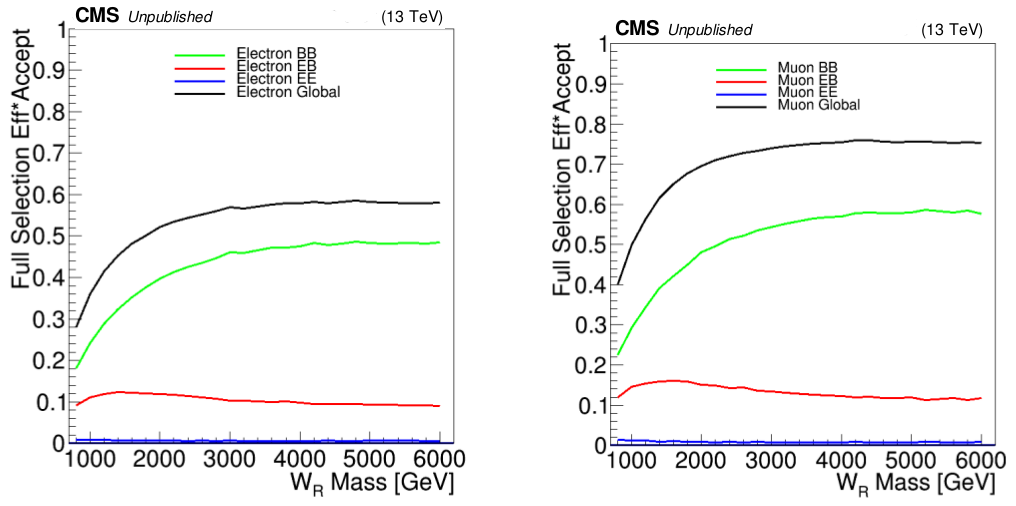
\includegraphics[width=1.0\textwidth]{figures/wrRecoSelectionEfficiency.png}
	\caption{The full selection efficiency in $\WR \rightarrow \ell\ell jj$ events, in the $ee$-channel ($\mu\mu$-channel) 
		on the left (right).  Different curves represent events where both leptons are in the barrel (BB), one was in the 
	endcap (EB), or both were in the endcap (EE).}
	\label{fig:wrRecoSelectionEff}
\end{figure}

After all selections, evidence of a \WR and \nul was searched for as an excess of events over expected backgrounds 
in one kinematic variable distribution.  The existence of a \WR and \nul would create an excess in many kinematic 
variable distributions, like the leading lepton $\pt$ distribution, but for most variables the shape, position, and 
magnitude of the excess is sensitive to the unknown masses \mWR and \mnul.  In addition, the event selections sculpted 
expected background events and created a peak away from $0$ in many kinematic variable distributions.  To avoid sculpted 
background distributions and mitigate sensitivity to \mWR and \mnul, evidence of a \WR and \nul was searched for as an 
excess in the $\Mlljj$ distribution.  There, evidence of a \WR would appear as a peak centered on \mWR 
that is distinguished from the $\Mlljj$ distribution expected from backgrounds, as shown in Figure \ref{fig:mlljjVariableOfMerit}.  
Before looking for evidence of a \WR and \nul in data, the $\Mlljj$ distribution expected from backgrounds was estimated 
using data and simulated events found in kinematic `control` regions where data and simulations were expected to agree.

\begin{figure}[h]
	\centering
	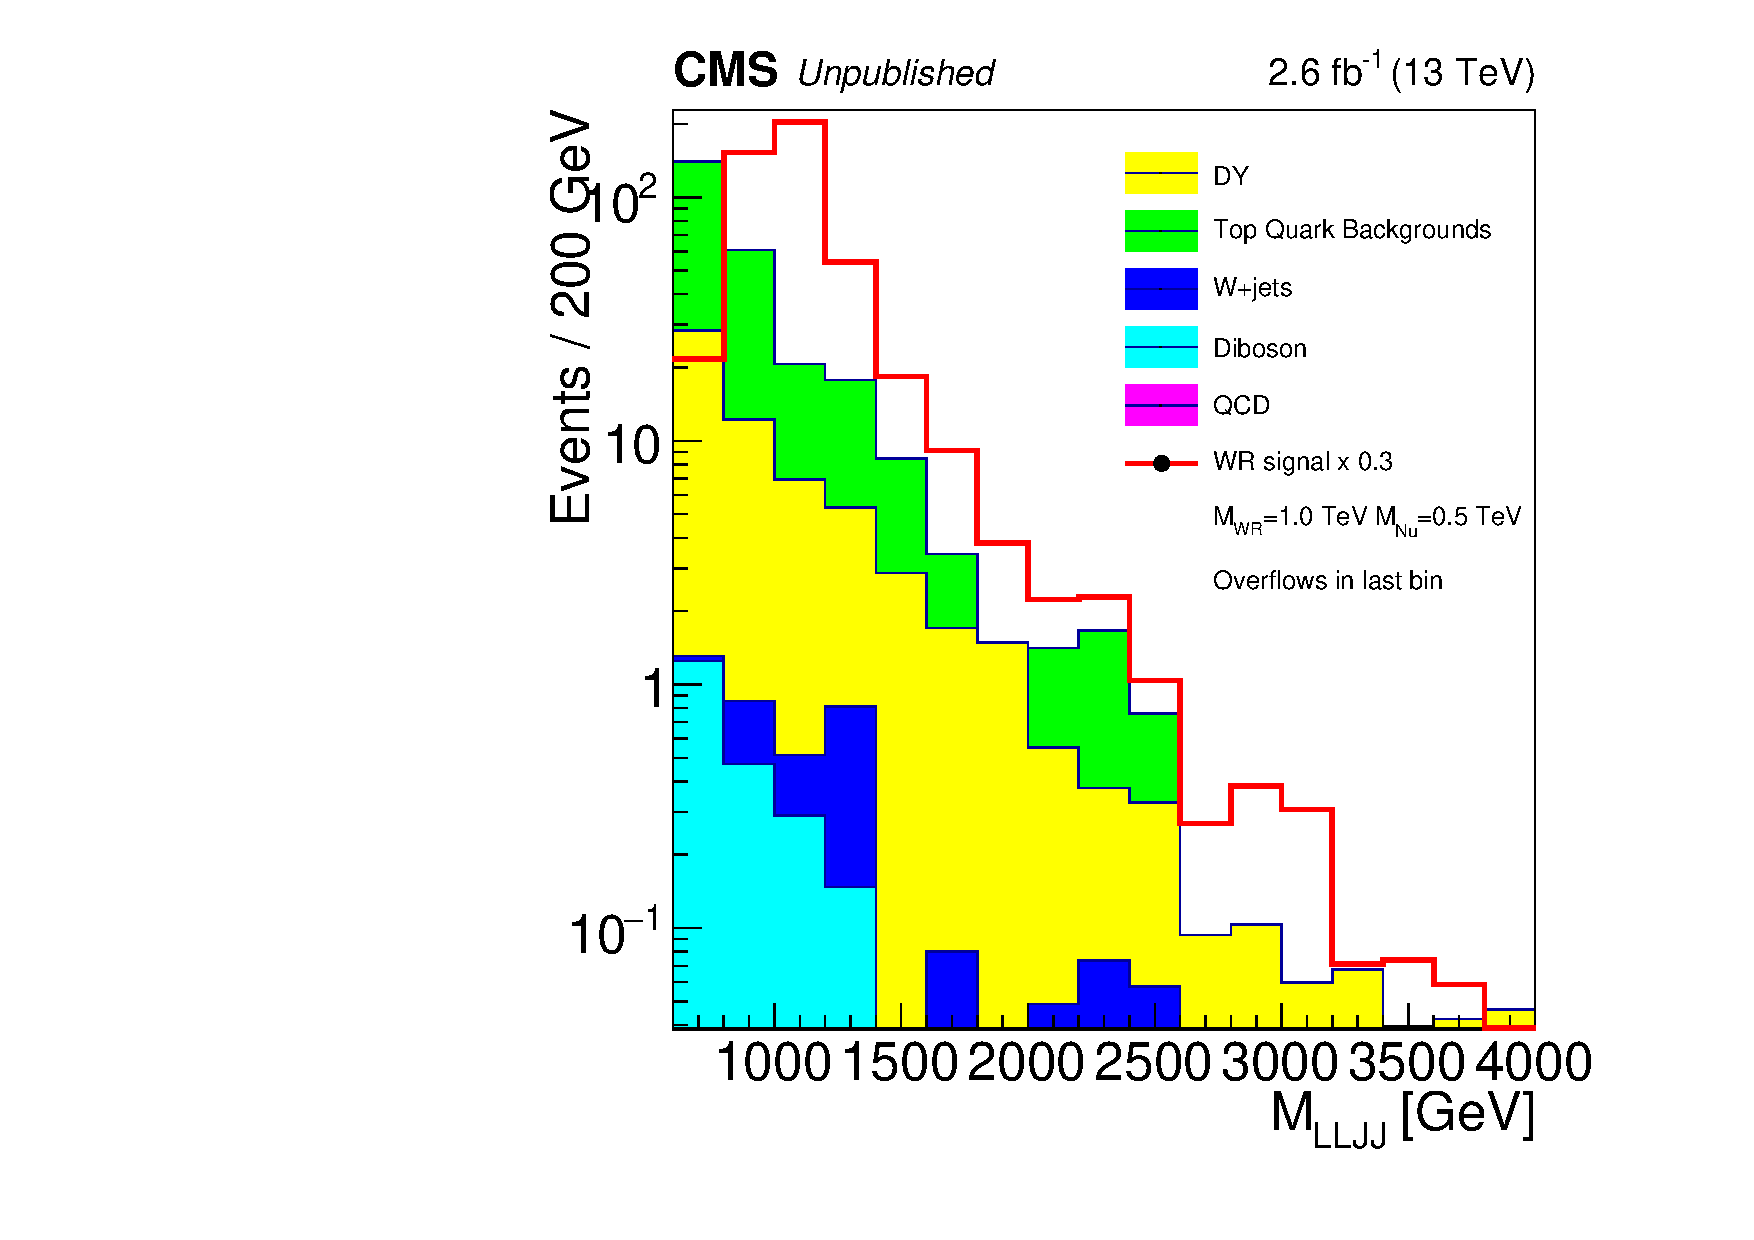
\includegraphics[width=0.7\textwidth]{figures/useOfLLJJMassAsFigureOfMerit.pdf}
	\caption{The $\Mlljj$ distribution from simulations of ST backgrounds and a \WR signal in the $ee$-channel.  
		The \WR signal normalization is reduced by 70\% to better visualize the difference 
	between the signal and expected backgrounds.}
	\label{fig:mlljjVariableOfMerit}
\end{figure}


%%%%%%%%%%%%%%%%%%%%%%%%%%%%%%%%%%%%%%%%%%%%%%%%%%%%%%%%%%%%%%%%%%%%%%%%%%%%%%%%
